\documentclass[bibtotoc,liststotoc,BCOR5mm,DIV12]{scrbook}

% use this declaration to set specific page margins
%\usepackage[a4paper , lmargin = {2.7cm} , rmargin = {2.9cm} , tmargin = {2.7cm} , bmargin = {4.6cm} ]{geometry}
\usepackage[a4paper]{geometry}
\usepackage{amsfonts}
\usepackage{amsmath}

\usepackage[ngerman, english]{babel}
%\usepackage{bibgerm}       		% german references
%\usepackage{natbib}

\usepackage{amsthm}
\theoremstyle{definition}
\newtheorem{definition}{Definition}[section]

\usepackage[latin1]{inputenc} % german characters
\usepackage{graphicx} 				% it's recommended to use PDF images but you can use JPG or PNG as well
\usepackage{url}           		% format URLs
\usepackage{hyperref} 				% create hyperlinks
\usepackage{listings, color}	% for source code
\usepackage{subfig}						% two figures next to each other (example: figure 3a), figure 3b)
\usepackage{scrpage2}					% header and footer line
\usepackage{ulem}
\usepackage{bbm}
\usepackage[ruled]{algorithm2e}
\usepackage{afterpage}
\usepackage{nomencl}
\makenomenclature


\usepackage{mfirstuc}


% header and footer line - no header & footer line on pages where a new chapter starts
\pagestyle{scrheadings}
\ohead{Designing Recurrent Neural Networks for Explainability}
\ihead{Pattarawat Chormai}
\ofoot[]{\thepage}
\usepackage{tikz}

%TODO : Footer : What is Fachgebiet? and 
%\ifoot{Master Thesis, TU Berlin, Fachgebiet ML, 2018}

% set path where images are stored
\graphicspath{{./img/}}


\addto{\captionsenglish}{%
  \renewcommand{\bibname}{References}
}

%TODO: Define commands
\newcommand{\addfigure}[1] {Figure #1}
\newcommand{\patmatrix}[1]{\boldsymbol{\uppercase{#1}}}
\newcommand{\patvector}[1]{\boldsymbol{\lowercase{#1}}}
\newcommand{\x}{\boldsymbol{x}}
\newcommand{\btheta}{\boldsymbol{\theta}}

\newcommand{\patarg}[2]{ \underset{#2}{\text{arg#1}}\   }


\newcommand*\circled[1]{\tikz[baseline=(char.base)]{
            \node[shape=circle,draw,inner sep=2pt, white, fill=red,minimum size=1em] (char) {\textbf{\footnotesize{#1}}};}}
            
\newcommand{\rnncellseq}[2]{\capitalisewords{#1}-#2}
\newcommand{\rnncell}[1]{\text{\capitalisewords{#1}}}
\newcommand{\todo}[1]{\textcolor{red}{TODO : #1}}
\newcommand{\xa}[0]{\patvector{x}^{(\alpha)}}
\newcommand{\ya}[0]{y^{(\alpha)}}
\newcommand{\yha}[0]{\hat{y}^{(\alpha)}}

  
%
% der Befehl \hypenation versteht keine Sonderzeichen, also weder �
% noch "a noch \"a. W�rter die derartige Zeichen enthalten m�ssen
% direkt im Text getrennt werden, z.B. W�r\-ter
%
\hyphenation{te-le-com-muni-cation 
te-le-com-muni-cation-specific 
Te-le-kom-mu-ni-ka-tions-API} 					% use this file to set explicit hyphenations (doesn't seem to work correctly)

\begin{document}
% ---------------------------------------------------------------
\frontmatter
    \thispagestyle{empty}
\begin{center}

{\LARGE \textbf{Technische Universit\"at Berlin}}

\vspace{0.5cm}

{\large Faculty IV : Electrical Engineering and Computer Science
\\[1mm]}
{\large Institute of Software Engineering and Theoretical Computer Science\\[5mm]}

Machine Learning Group\\
Marchstr. 23\\
10587 Berlin\\

\vspace*{1cm}


\includegraphics[width=4cm]{tu_logo.jpg}

\vspace*{1.0cm}

{\LARGE{Master Thesis} }

\vspace{1.0cm}
{\LARGE \textbf{Designing Recurrent Neural Networks}}\\
\vspace*{0.3cm}
{\LARGE \textbf{ for Explainability}}\\
\vspace*{1.0cm}
{\LARGE Pattarawat Chormai}
\\
\vspace*{0.5cm}
Matriculation Number: 387441\\
\today  \\ % 	date of submission

\vspace*{1.0cm}

\textbf{Supervised by}\\
Prof. Dr. Klaus-Robert M\"{u}ller \\
Dr. Gr\'{e}goire Montavon
%\vspace*{0.5cm}
%\textbf{Advisor}\\


\vspace{3cm}


\end{center}


   	\thispagestyle{empty}
    \cleardoublepage
    
    \thispagestyle{empty}
\vspace*{3cm}
\begin{center}
    \textbf{Acknowledgement}
\end{center}

% todo : Writing Acknoeledgement
First of all, I would like to thank Prof. Dr. Klaus-Robert M\"{u}ller and Dr. Gr\'{e}goire Montavon for this research opportunity and invaluable guidance throughout  the course of conducting the thesis as well as facilitating me at TU Berlin, Machine Learning group with a great research environment . I would also like to thank Prof. Dr. Klaus Obermayer and staffs of Neural Information Processing group for organizing Machine Intelligence I \& II and Neural Information Project. These courses provide me necessary knowledge to conduct the thesis.


Secondly, I would like to thank to my family for always providing me financial and mental support. 

Thanks EIT colleagues and . In particular, Someone for proofreading..

I would like to thank EIT Master School as well as TU/e and TUB staffs that involve in this study program.  Your support and advice are always helpful. 

Lastly, I would like to acknowledge Amazon AWS for generous educational credits and Auction Club S.a.r.L, Luxembourg for lending me a powerful laptop to use in my study. None of experiments would have been possible without these computational resource supports.
    \thispagestyle{empty}
    \cleardoublepage
    
    \newpage

\thispagestyle{empty}

\begin{large}

\vspace*{6cm}

\noindent
Hereby I declare that I wrote this thesis myself with the help of no more than the mentioned literature and auxiliary means.
\vspace{2cm}

\noindent
Berlin, 01.01.2050

\vspace{3cm}

\hspace*{7cm}%
\dotfill\\
\hspace*{8.5cm}%
\textit{(Signature [your name])}

\end{large}
 
    \thispagestyle{empty}
    \cleardoublepage
    
    
    \thispagestyle{empty}
\vspace*{1.0cm}

\begin{center}
    \textbf{Abstract}
\end{center}

\vspace*{0.5cm}

\noindent
%TODO Writing abstract 
Standard (non-LSTM) recurrent neural networks have been challenging to train, but special optimization techniques such as heavy momentum makes this possible. However, the potentially strong entangling of features that results from this difficult optimization problem can cause deep Taylor or LRP-type to perform rather poorly due to their lack of global scope. LSTM networks are an alternative, but their gating function make them hard to explain by deep Taylor LRP in a fully principled manner. Ideally, the RNN should be expressible as a deep ReLU network, but also be reasonably disentangled to let deep Taylor LRP perform reasonably. The goal of this thesis will be to enrich the structure of the RNN with more layers to better isolate the recurrent mechanism from the representational part of the model. 
    \thispagestyle{empty}
    \cleardoublepage
    
   % TODO German abstract?
    \thispagestyle{empty}
\vspace*{0.2cm}

\begin{center}
    \textbf{Zusammenfassung}
\end{center}

\vspace*{0.2cm}

\noindent 
Da die meisten Leuten an der TU deutsch als Muttersprache haben, empfiehlt es sich, das Abstract zus�tzlich auch in deutsch zu schreiben. Man kann es auch nur auf deutsch schreiben und anschlie�end einem Englisch-Muttersprachler zur �bersetzung geben.
    \thispagestyle{empty}
    
    
    
    
    \tableofcontents
    \thispagestyle{empty}
    
    \thispagestyle{empty}
\addcontentsline{toc}{chapter}{Notation}

%\vspace*{0.2cm}

%\begin{center}
%    \textbf{Mathematical Notation}
%\end{center}

%\vspace*{0.2cm}
\renewcommand{\nomname}{Notation}
\setlength{\nomlabelwidth}{3cm}

\printnomenclature
\nomenclature{$a_j$}{Activation of neuron $j$}
\nomenclature{$b_k$}{Bias of neuron $k$}
\nomenclature{$x_i$}{Feature $i$ of input sample $x$}
\nomenclature{$w_{jk}$}{Weight between neuron $j$ to neuron $k$} 
\nomenclature{$R_j$}{Relevance score of neuron $j$} 
\nomenclature{$R_{j \leftarrow k }$}{Relevance score distributed from neuron $k$ to neuron $j$} 
\nomenclature{$\sigma$}{An activation function}
\nomenclature{$\{ a_j \}_L$}{A vector of activations of neurons in layer $L$}
\nomenclature{$\patvector{x}, \patvector{x}^{(\alpha)}$}{A vector representing an input sample} 
\nomenclature{$\patvector{\theta}$}{Parameters of a neural network} 

%\nomenclature{$R(\patvector{x})$}{Relevance heatmap of $\patvector{x}$} 
    
    \listoffigures
    \thispagestyle{empty}
    
    \listoftables
    \thispagestyle{empty}
    

    
% --------------------------------------------------------------

\mainmatter % comment single chapters for faster compilation

    \chapter{Introduction}
\label{cha:chapter1}
In recent years, machine learning (ML) has been increasingly involved in almost every aspect of our life, for example, recommendation systems on e-commerce sites, medical diagnosis, or self-driving cars. This development cannot be achieved without intelligent algorithms behind. A particular type of ML algorithms, called neural networks (NNs), have been gradually used to power such systems.  This is because NNs have directly benefitted from the vast amount of data available and more efficient computation resources developed, giving a much better performance as compared to other ML algorithms. As a result, intelligent systems we use nowadays frequently rely on them.

In short, NNs are algorithms inspired by how the human brain works. One of their advantages is that they can learn patterns from data efficiently. NNs comprise of simple units, called neurons, arranged in layers working together to transform input to the desired output. When the network is comprised of many layers, it is often referred to as \textit{deep learning}. Connections between neurons define this transformation. These connections are learned from the training data without being explicitly defined. 

Because the transformation is typically non-linear in a high dimensional space and built to a specific problem, it is not apparent to us how the trained NN utilizes input and makes a prediction.  This lack of this understanding raises concerns and questions to the machine learning community and stakeholders. One primary concern is about trust, in particular, how we can ensure that trained NNs will work as we expect. Secondly, not having this insight results in considerable amount of trials and errors when it comes to adjusting configurations of NNs to achieve better performance.

Researchers have proposed several methods to better understand or explain how NNs transform input to output. In particular, \citet{SimonyanDeepConvolutionalNetworks2013}  proposed a pioneer work in understanding predictions of NNs through the \textit{activation maximization} approach and a method relying on partial derivatives which we refer to as \textit{sensitivity analysis} (SA). \citet{SpringenbergStrivingSimplicityAll2015a} suggested a modified version of SA, called \textit{guided backprop} (GB), for ReLU-type NNs. In the results, GB produces more informative explanations than SA. \citet{SmilkovSmoothGradremovingnoise2017}  proposed the \textit{SmoothGrad} technique to improve quality of SA explanations. 

\cite{BachPixelWiseExplanationsNonLinear2015} proposed an alternative approach, called \textit{Layer-wise Relevance Propagation} (LRP). The method utilizes the architecture of the NN itself to create explanations, instead of relying on partial derivatives as in SA and GB. For ReLU-type networks, \citet{MontavonExplainingnonlinearclassification2017} derived  the \textit{deep Taylor decomposition} (DTD) technique for explaining their non-linear decisions. They showed that DTD is a special case of LRP. \citet{SundararajanAxiomaticAttributionDeep2017a} proposed the \textit{integrated gradients} method combining gradient and decomposition techniques. \citet{RibeiroWhyShouldTrust2016} developed the \textit{Local Interpretable Model-Agnostic Explanations} (LIME) framework that can explain predictions of a wider set of models. \citet{OlahBuildingBlocksInterpretability2018} suggested ideas for visualizing explanations from multiple domains. 

These works have primarily focused on standard NNs or feedforward architectures. However, there is still only a limited number of contributions in explaining predictions from recurrent neural networks (RNNs). RNNs are essential algorithms in domains that process sequential data, such as machine translation and natural language processing (NLP). To the best of our knowledge, the closest works in this direction are from 1) \citet{KarpathyVisualizingUnderstandingRecurrent2015} that  interpreted activations of LSTM \citep{HochreiterLongshorttermmemory1997} cells for a certain task and 2) \citet{ArrasExplainingRecurrentNeural2017} that applied LRP to a LSTM network trained to perform a sentiment analysis task. Therefore, a study of explaining RNN predictions needs to be further explored. This study will enable us to gain insight how RNNs internally work and hopefully it will lead us to developments of more explainable RNNs.


%In fact, state-of-the-art of these applications today mostly rely on RNN. However, the question of how neural networks, including RNN, derive their predictions is still unclear to us. This causes resistance in the adoptation and development of the technology itself. 

%
%
%However, there is still only few work in the direction of explaining predictions from RNN. 
%
%
% Although these work has demonstrated promising results on neural networks, more specifically feed-forward architectures, there is still only a few applications of these methods to recurrent architecture. These recurrent neural networks are considerably important and have been powering almost machine learning systems processing sequential data, such as machine translation and natural language understanding. Therefore, applications of these explanation techniques to recurrent neural networks need to be explored. This results will also enable us to propose adjustments to recurrent architectures such that they are more explainable.


\section{Objective \& Scope}
This thesis aims to explain RNN predictions. More precisely, the goal of this thesis is to study how the architecture of RNNs affects the quality of explanations produced by various explanation techniques. In particular, we are interested in applying explanation techniques that were developed for feedforward architectures, such as sensitivity analysis, guided backprop, Layer-wise Relevance Propagation and deep Taylor decomposition to the RNN setting. 

Our study is based on artificial classification problems using MNIST and FashionMNIST dataset. These problems are specially constructed such that the ground truth explanation knowledge is available to us. As a result, we can perform qualitative and quantitative measurements accordingly.


We hypothesize that RNNs with more layers are more explainable than ones with fewer layers. We conduct extensive experiments on various configurations to verify our proposition. We also propose an adjustment to the LSTM architecture. The adjustment allows us to apply the explanation techniques to the architecture.

Lastly, because we consider the harder case where data arrives sequentially and not all at once like convolutional neural networks (CNNs), classification accuracy is limited by this more challenging setting. Therefore, we do not seek to train models to achieve the state-of-the-art performance. We instead train them to reach a certain level of accuracy. We assume that models operating at this level are good enough and produce comparable explanations. 
%
%as the primary goal is to study explainability of RNNs, it is worth mentioning that we do not seek to train models to achieve the state-of-the-art performance. We instead train them to reach a certain level of accuracy. We assume that models operating at this level are good enough and produce comparable explanations. In fact, the classification problems we are considering are harder cases because data arrives sequentially and not all at once like convolutional neural networks (CNNs). Therefore, classification accuracy is limited by this more challenging setting. 


%assumption relu? ... 
%
%not care performance much ..
%
%our hypothesis ... 
%
%artificial problems ... 


%\section{Dataset}
%Our study is based on MNIST\citep{LeCunMNISThandwrittendigit2010} and FashionMNIST\citep{XiaoFashionMNISTNovelImage2017}. Following is a brief introduction of them.
%
%\subsection{MNIST}
%
%\begin{figure}[!hbt]
%	\centering
%	
\includegraphics[width=0.6\textwidth]{mnist}
%	\caption{MNIST dataset.}
%	\label{fig:mnist_samples}
%\end{figure}
%
%MNIST is one of the most popular dataset that machine learning partitioners use to benchmark machine learning algorithms. The dataset consists of 60,000 training and 10,000 testing samples. Each sample is a grayscale 28x28 image. As shown in \addfigure{\ref{fig:mnist_samples}}, MNIST has 10 categories corresponding to a digit between 0 and 9.
%
%
%State-of-the-art algorithms can classify MNIST with accuracy higher than 99\%, while classical ones, such as SVC or RandomForest, are able to achieve around 97\%\citep{XiaoFashionMNISTNovelImage2017}.
%
%
%\subsection{FashionMNIST}
%
%FashionMNIST is a dataset \todo{ rephrase : whose authors aim to it to be a replacement of MNIST, especially in  benchmarking machine learning algorithms}.  According to \citep{XiaoFashionMNISTNovelImage2017},  FashionMNIST is more representative to modern computer vision tasks. It contains images of fashion products from 10 categories and compatible  to MNIST in every aspects, such as the size of training and testing set, image dimension and data format, hence one can easily  apply existing algorithms that work with MNIST to Fashion-MNIST without any change. \addfigure{\ref{fig:fashion_mnist_samples}} shows FashionMNIST samples.
%
%\begin{figure}[!hbt]
%\centering
%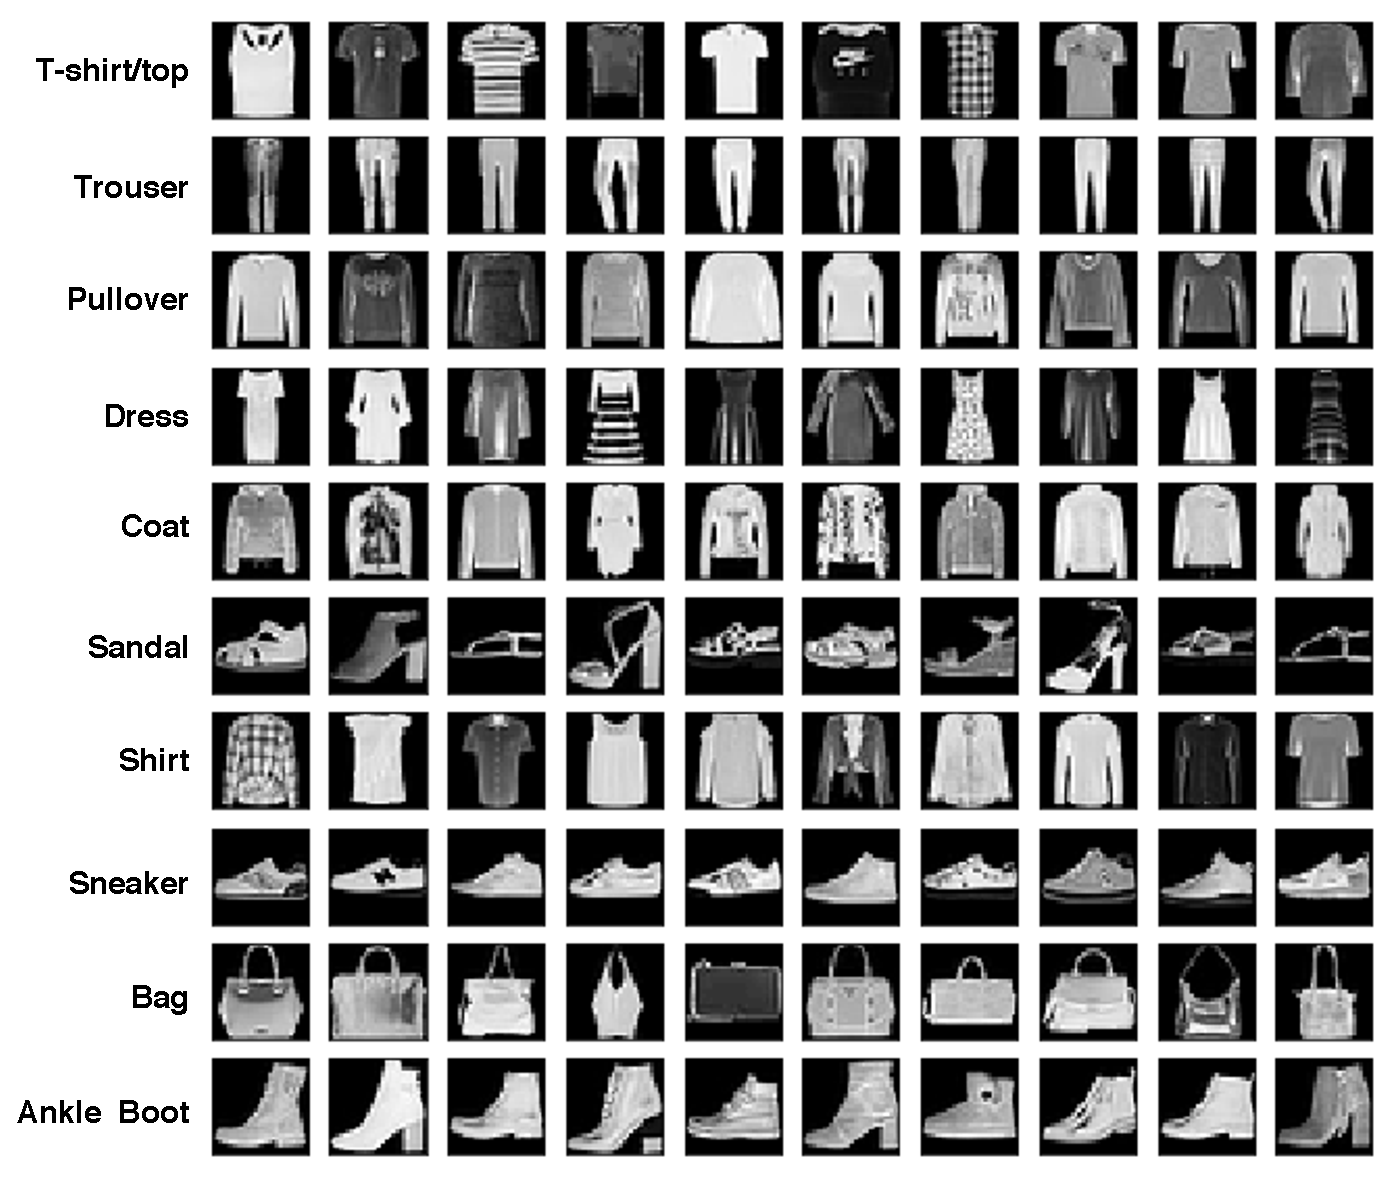
\includegraphics[width=0.65\textwidth]{sketch/fmnist_samples}
%\caption{FashionMNIST dataset.}
%\label{fig:fashion_mnist_samples}
%\end{figure}
%
%\citet{XiaoFashionMNISTNovelImage2017} also reports benchmarking results of classical machine learning algorithms on Fashion-MNIST. On average, they achieve accuracy between 85\% to 89\%. According to Fashion-MNIST's page\footnote{https://github.com/zalandoresearch/fashion-mnist}, state-of-the-art result has 97\% accuracy using Wide Residual Network(WRN)\citep{ZagoruykoWideResidualNetworks2016} and standard data preprocessing and augmentation.

%\section{Terminology}
%\todo{terminology}

\clearpage

\section{Outline}
The thesis is organized as follows:
\begin{itemize}
%	\item \textbf{Chapter \ref{cha:chapter2}} provides a brief literature survey and related work in the direction towards explaining neural networks.
	\item \textbf{Chapter \ref{cha:chapter3}} summarizes relevant topics in  neural networks and explanation techniques that are focused in the thesis.
	\item \textbf{Chapter \ref{cha:chapter4}} is devoted to experimental results.
	\item \textbf{Chapter \ref{cha:chapter5}} concludes the results and discusses challenges as well as future work.
\end{itemize}

%
%This chapter should have about 4-8 pages and at least one image, describing your topic and your concept. Usually the introduction chapter is separated into subsections like 'motivation', 'objective', 'scope' and 'outline'.
%
%\section{Motivation\label{sec:moti}}
%
%Start describing the situation as it is today or as it has been during the last years. 'Over the last few years there has been a tendency... In recent years...'. The introduction should make people aware of the problem that you are trying to solve with your concept, respectively implementation. Don't start with 'In my thesis I will implement X'.
%
%\section{Objective\label{sec:objective}}
%
%What kind of problem do you adress? Which issues do you try to solve? What solution do you propose? What is your goal?
%'This thesis describes an approach to combining X and Y... The aim of this work is to...'
%
%\section{Scope\label{sec:scope}}
%
%Here you should describe what you will do and also what you will not do. Explain a little more specific than in the objective section. 'I will implement X on the platforms Y and Z based on technology A and B.'
%
%Conclude this subsection with an image describing 'the big picture'. How does your solution fit into a larger environment? You may also add another image with the overall structure of your component.
%
%'Figure \ref{fig:intro} shows Component X as part of ...' 
%\\
%\begin{figure}[htb]
%  \centering
%  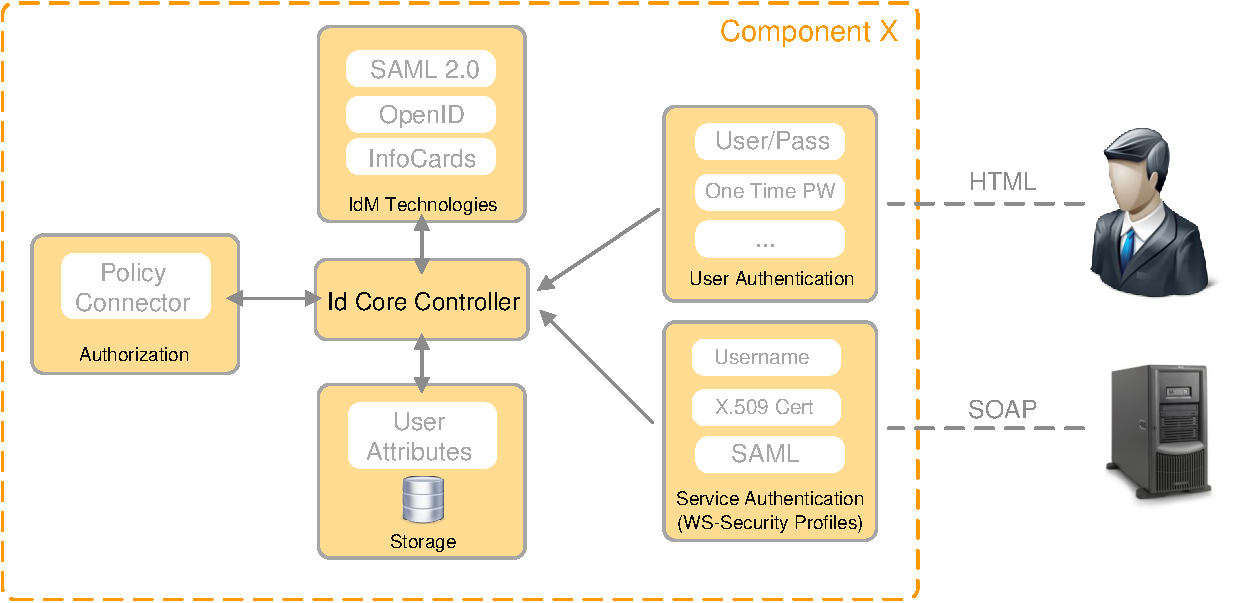
\includegraphics[width=9cm]{intro_example.pdf}\\
%  \caption{Component X}\label{fig:intro}
%\end{figure}
%
%\section{Outline\label{sec:outline}}
%
%The 'structure' or 'outline' section gives a brief introduction into the main chapters of your work. Write 2-5 lines about each chapter. Usually diploma thesis are separated into 6-8 main chapters. 
%\\
%\\
%\noindent This example thesis is separated into 7 chapters.
%\\
%\\
%\textbf{Chapter \ref{cha:chapter2}}  Neural Network and Explainability foudation
%%is usually termed 'Related Work', 'State of the Art' or 'Fundamentals'. Here you will describe relevant technologies and standards related to your topic. What did other scientists propose regarding your topic? This chapter makes about 20-30 percent of the complete thesis.
%\\
%\\
%\textbf{Chapter \ref{cha:chapter3}} Architecture
%%analyzes the requirements for your component. This chapter will have 5-10 pages.
%\\
%\\
%\textbf{Chapter \ref{cha:chapter4}} Experiments
%%Ais usually termed 'Concept', 'Design' or 'Model'. Here you describe your approach, give a high-level description to the architectural structure and to the single components that your solution consists of. Use structured images and UML diagrams for explanation. This chapter will have a volume of 20-30 percent of your thesis.
%\\
%\\
%\textbf{Chapter \ref{cha:chapter5}} Conclusion and future work
%%describes the implementation part of your work. Don't explain every code detail but emphasize important aspects of your implementation. This chapter will have a volume of 15-20 percent of your thesis.
%%\\
%\\
%%\textbf{Chapter \ref{cha:chapter6}} is usually termed 'Evaluation' or 'Validation'. How did you test it? In which environment? How does it scale? Measurements, tests, screenshots. This chapter will have a volume of 10-15 percent of your thesis.
%%\\
%%\\
%%\textbf{Chapter \ref{cha:chapter7}} summarizes the thesis, describes the problems that occurred and gives an outlook about future work. Should have about 4-6 pages.
      \chapter{Fundamentals and Related Work\label{cha:chapter2}}

This section is intended to give an introduction about relevant terms, technologies and standards in the field of X. You do not have to explain common technologies such as HTML or XML. 

\section{Technologies \label{sec:tech}}

This section describes relevant technologies, starting with X followed by Y, concluding with Z.

\subsection{Technology A\label{sec:aaa}}

It's always a good idea to explain a technology or a system with a citation of a prominent source, such as a widely accepted technical book or a famous person or organization. 

Exmple: Tim-Berners-Lee describes the ''WorldWideWeb'' as follows:
\\
\textit{''The WorldWideWeb (W3) is a wide-area hypermedia information retrieval initiative aiming to give universal access to a large universe of documents.''} \cite{timwww}
\\
\\
You can also cite different claims about the same term.
\\
According to Bill Gates \textit{''Windows 7 is the best operating system that has ever been released''} \cite{billgates} (no real quote)
In opposite Steve Jobs claims Leopard to be \textit{''the one and only operating system''} \cite{stevejobs}

If the topic you are talking about can be grouped into different categories you can start with a classification.
Example: According to Tim Berners-Lee XYZ can be classified into three different groups, depending on foobar \cite{timwww}:
	\begin{itemize}
		\item Mobile X
				\vspace{-0.1in} 
		\item Fixed X
				\vspace{-0.1in} 
		\item Combined X
 	\end{itemize}

\subsection{Technology B\label{sec:bbb}}

For internal references use the 'ref' tag of LaTeX. Technology B is similar to Technology A as described in section \ref{sec:aaa}.

\newpage

\subsection{Comparison of Technologies\label{sec:comp}}

\begin{table}[htb]
\centering
\begin{tabular}[t]{|l|l|l|l|}
\hline
Name & Vendor & Release Year & Platform \\
\hline
\hline
A & Microsoft & 2000 & Windows \\
\hline
B & Yahoo! & 2003 & Windows, Mac OS \\
\hline
C & Apple & 2005 & Mac OS \\
\hline
D & Google & 2005 & Windows, Linux, Mac OS \\
\hline
\end{tabular}
\caption{Comparison of technologies}
\label{tab:enghistory}
\end{table}

\section{Standardization \label{sec:standard}}

This sections outlines standardization approaches regarding X.

\subsection{Internet Engineering Task Force\label{sec:itu}}

The IETF defines SIP as '...' \cite{rfcsip}

\subsection{International Telecommunication Union\label{sec:itu}}

Lorem Ipsum...

\subsection{3GPP\label{sec:3gpp}}

Lorem Ipsum...

\subsection{Open Mobile Alliance\label{sec:oma}}

Lorem Ipsum...

\section{Concurrent Approaches \label{sec:summ}}

There are lots of people who tried to implement Component X. The most relevant are ...

    \chapter{Requirements\label{cha:chapter3}}
This section determines the requirements necessary for X. This includes the functional aspects, namely Y and Z, and the non functional aspects such as A and B.

\section{Overview\label{sec:reqoverview}}

In this chapter you will describe the requirements for your component. Try to group the requirements into subsections such as 'technical requirements', 'functional requirements', 'social requirements' or something like this. If your component consist of different partial components you can also group the requirements for the corresponding parts. 

Explain the source of the requirements. 

Example: The requirements for an X have been widely investigated by Organization Y. 

In his paper about Z, Mister X outlines the following requirements for a Component X.

\section{Technical Requirements\label{sec:techreq}}

The following subsection outlines the technical requirements to Component X.

\subsection{Sub-component A\label{sec:reqsuba}}

\textbf{Interoperability}
\\
Lorem Ipsum...
\\
\\
\textbf{Scalability}
\\
Lorem Ipsum...

\subsection{Sub-component B\label{sec:reqsubb}}

Lorem Ipsum...

\section{Social Requirements\label{sec:socreq}}

Component X must compete with Y. Hence, it is required to provide an excellent usability. This includes ...
    \chapter{Experiments}
\label{cha:chapter4}

\section{Dataset}


\subsection{MNIST}
MNIST\cite{LeCunMNISThandwrittendigit2010} is one of the most popular dataset that machine learning partitioners use to benchmark machine learning algorithms. The dataset consists of 60,000 training and 10,000 testing samples. Each sample is a grayscale 28x28 image of a digit between from 0 to 9. 

\begin{figure}[h]
\centering

\includegraphics[width=0.5\textwidth]{mnist}
\caption{MNIST Dataset}
\label{fig:mnist_samples}
\end{figure}

State-of-the-art algorithms can classify MNIST with accuracy higher than 0.99, while classical ones, such as SVC or RandomForest, are able to achieve around 0.97\cite{XiaoFashionMNISTNovelImage2017}.


\subsection{Fashion-MNIST}

Xiao et. al.\cite{XiaoFashionMNISTNovelImage2017} propose a novel dataset, called Fashion-MNIST dataset, as a replacement of MNIST dataset for benchmarking machine learning algorithms.  According to \cite{XiaoFashionMNISTNovelImage2017},  Fashion-MNIST brings more challenging to the problem and more representative to modern computer vision tasks. It contains images of fashion products from 10 categories. Fashion-MNIST is comparable to MNIST in every aspects, such as the size of training and testing set, image dimension and data format, hence one can easily  apply existing algorithms that work with MNIST to Fashion-MNIST without any change.

\begin{figure}[h]
\centering
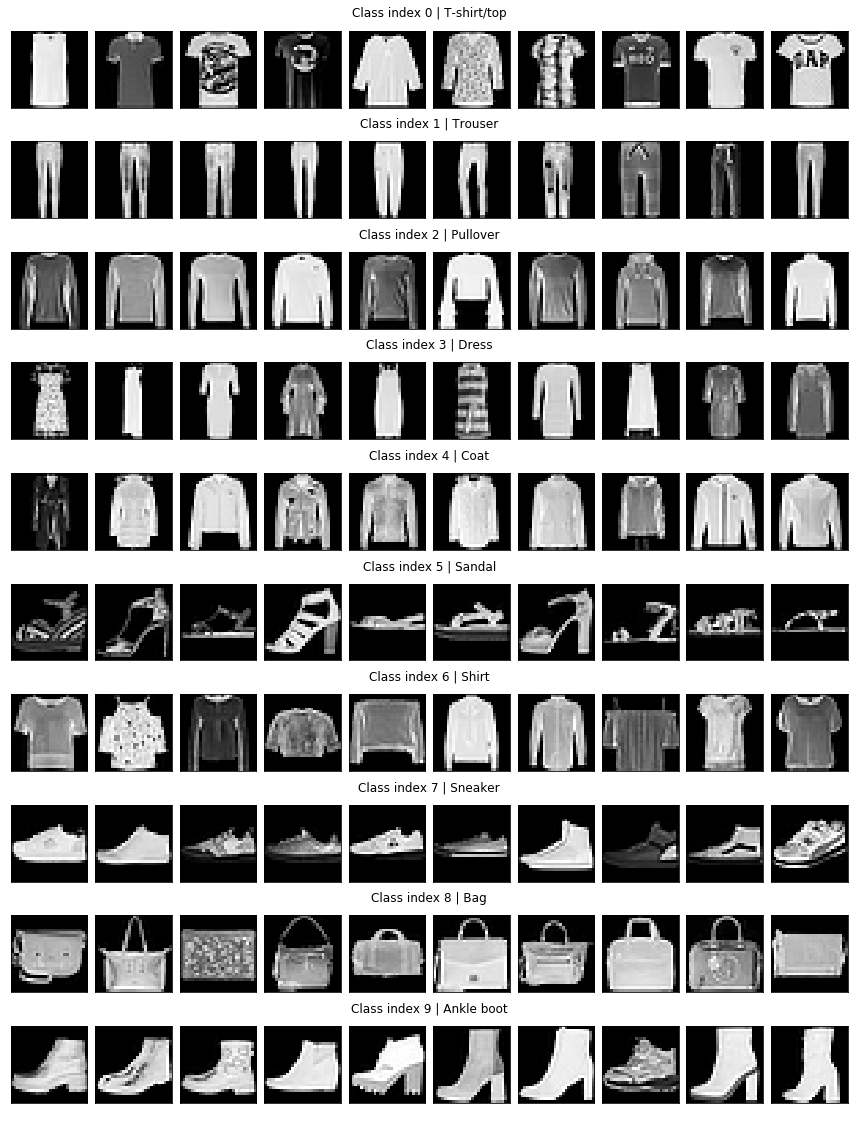
\includegraphics[width=0.6\textwidth]{fashion_mnist}
\caption{Fashion-MNIST Dataset\todo{Figure use same size as MNIST figure}}
\label{fig:fashion_mnist_samples}
\end{figure}

\cite{XiaoFashionMNISTNovelImage2017} also reports benchmarking results of classical machine learning algorithms on Fashion-MNIST. On average, they achieve accuracy between 0.85 to 0.89. According to Fashion-MNIST's page\footnote{https://github.com/zalandoresearch/fashion-mnist}, A. Brock reports the state-of-the-art result  with 0.97 accuracy using Wide Residual Network(WRN)\cite{ZagoruykoWideResidualNetworks2016} and standard data preprocessing and augmentation.


\section{RNN Cell Architectures}
In this section, I will describe architectures or RNN cell evaluated in this thesis.  To make the descriptions concise, I denote notations as follows: 

\begin{itemize}
	\item $\patvector{a}_{t}^{(l)}$ : activation vector of layer $l$ at step $t$
	\item $\patvector{x}_t$ : subset of $x_i \in \patvector{x}$ corresponding to step $t$ and assume to be reshaped into a column vector
\end{itemize}

\subsection{Shallow Cell}
\begin{figure}[!htb]
\centering

\subfloat[Shallow cell\label{fig:s2_network}]{%
       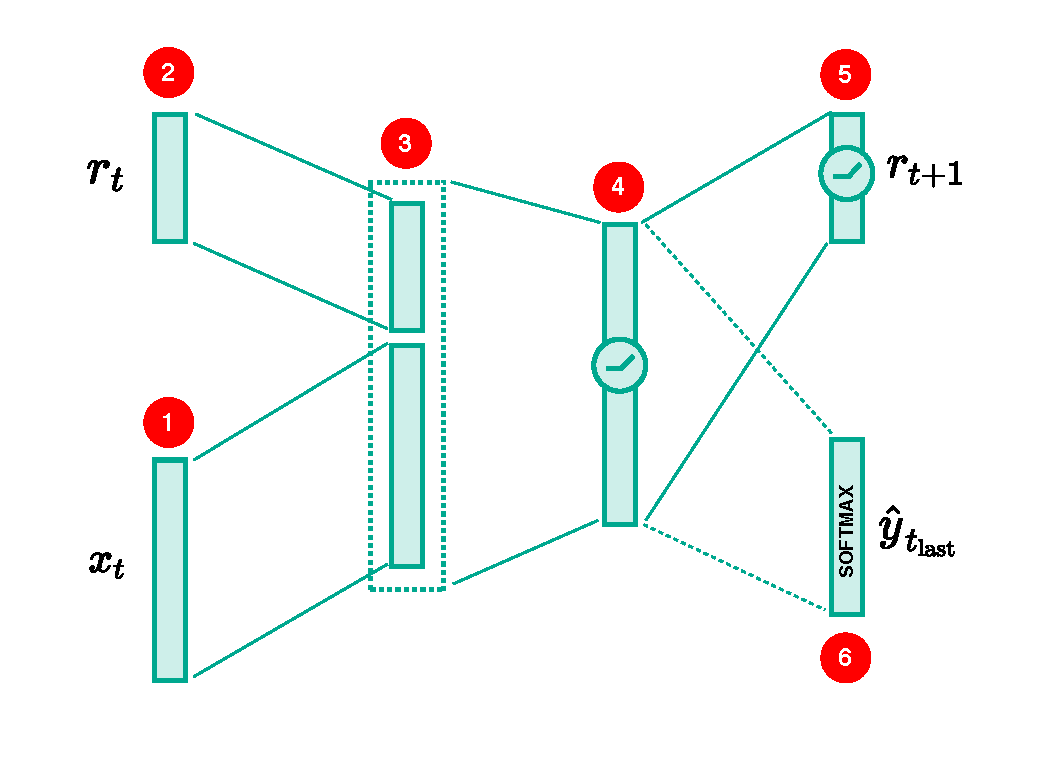
\includegraphics[width=0.48\textwidth]{sketch/s2_network}
     }
     \hfill
     \subfloat[Deep cell\label{fig:s3_network}]{%
       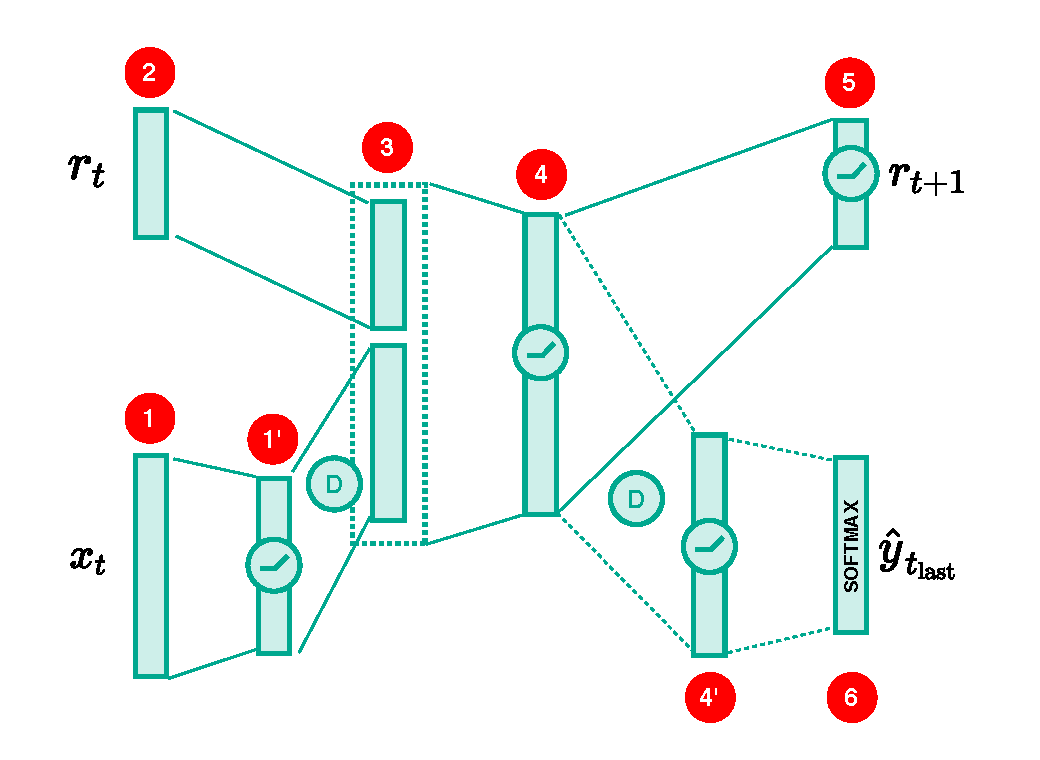
\includegraphics[width=0.48\textwidth]{sketch/s3_network}
     }
\caption{Shallow and Deep Cell Architecture}
\end{figure}

As shown in \addfigure{\ref{fig:s2_network}}, \rnncell{Shallow} cell first concatenates  input $\patvector{x}_t$  \circled{1} and recurrent input $\patvector{r}_t$  \circled{2} at layer \circled{3} as one vector before computing $\patvector{a}_t^{(4)} $ of layer \circled{4}. Then,  the next recurrent input $\patvector{r}_{t+1}$ \circled{5}	 is derived from $\patvector{a}_t^{(4)}$. In the last step $t_{\text{last}}$, the raw output $\patvector{h}$ is computed from $\patvector{a}^{(4)}_{t_{\text{last}}}$ and applied to softmax function to compute class probabilities $\patvector{\hat{y}}$ \circled{6}.



\subsection{Deep Cell Architecture}
%\begin{figure}[!htb]
%\centering
%
%\end{figure}

\addfigure{\ref{fig:s3_network}} illustrates the architecture of  \rnncell{Deep} cell. It can be viewed as  an extension of the Shallow cell with  2 additional layers, namely \circled{1'} and \circled{4'}.  The ideas of introducing the layers are to let \circled{1'} learn representations of the problem, while \circled{4} can focus on combining information from past and current step, which enables \circled{4'} to compute more fine-grained decision probabilities. Dropout is applied at $\patvector{a}^{(1')}_{\cdot}$, and $\patvector{a}^{(4)}_{t_\text{last}}$ for computing $\patvector{a}^{(4')}$.

\begin{figure}[!htb]
\centering

\subfloat[DeepV2\label{fig:deep_4l_network}]{%
       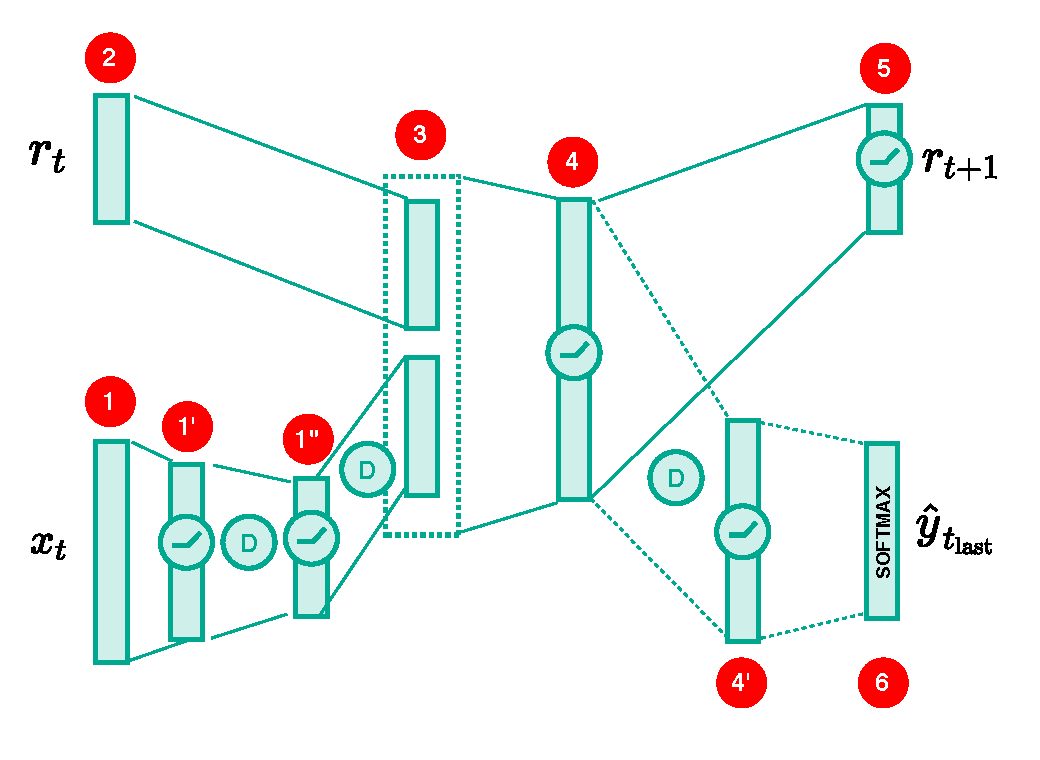
\includegraphics[width=0.48\textwidth]{sketch/deep_4l_network}
     }
     \hfill
     \subfloat[ConvDeep\label{fig:convdeep_4l_network}]{%
       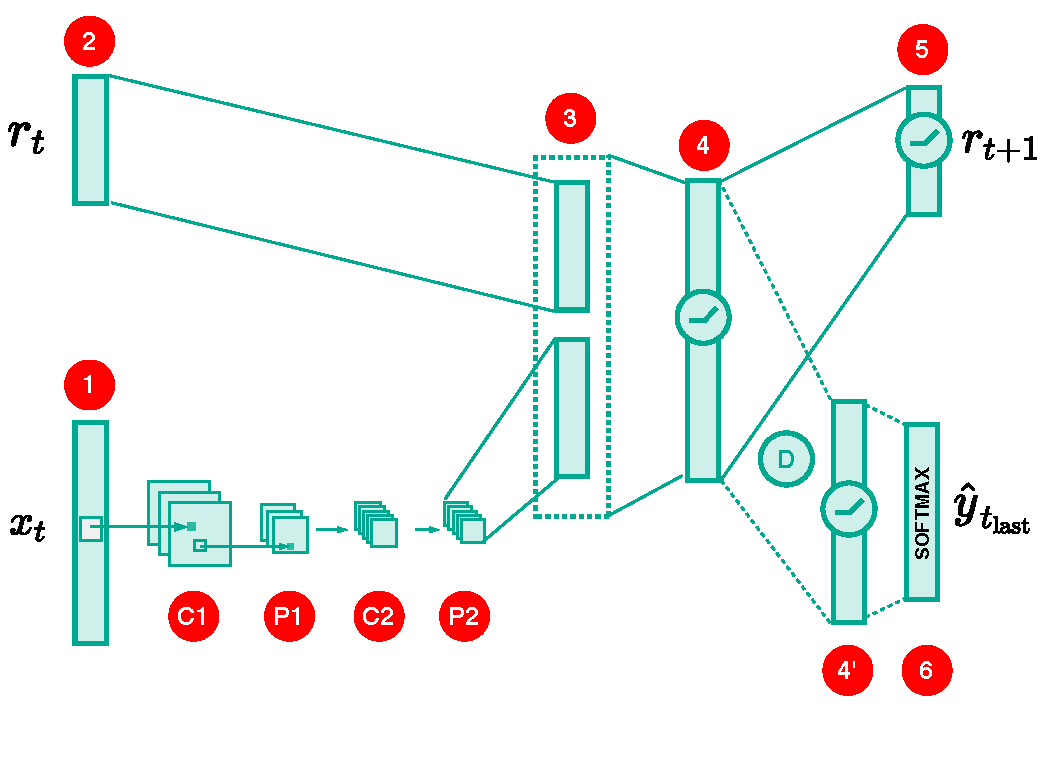
\includegraphics[width=0.48\textwidth]{sketch/convdeep_4l_network}
     }

\caption{DeepV2 and ConvDeep Cell Architecture}
\label{fig:deep_conv_arch}
\end{figure}
%
%
%
%\begin{figure}[!htb]
%\centering
%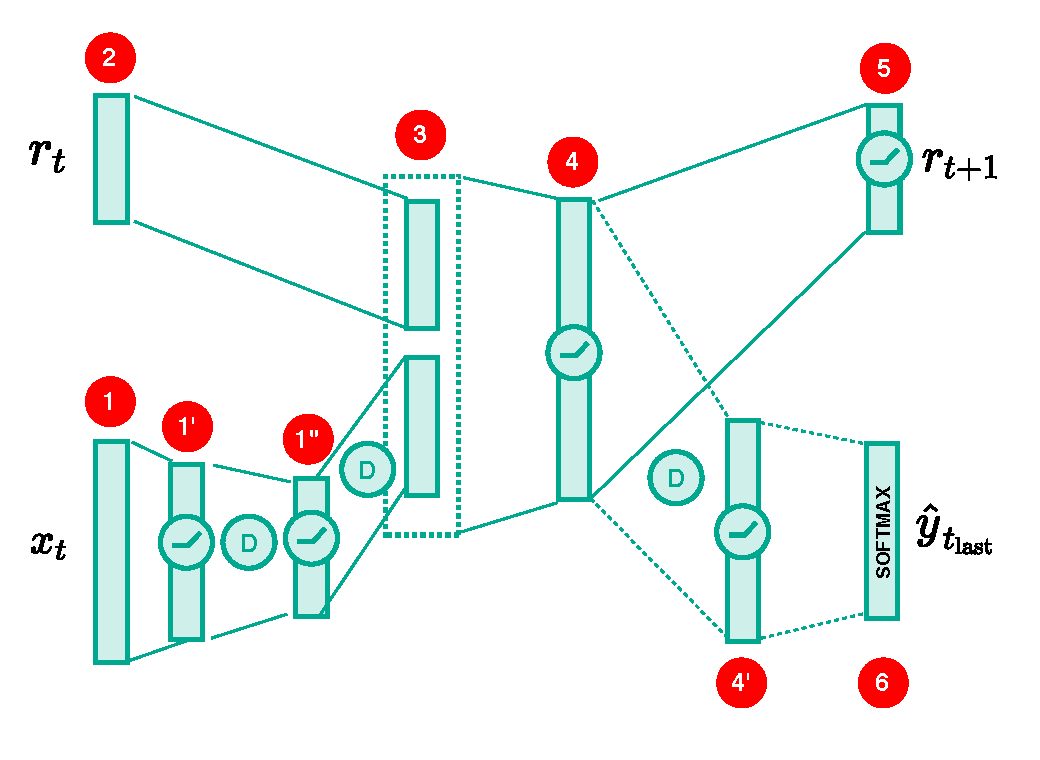
\includegraphics[width=0.6\textwidth]{sketch/deep_4l_network}
%\caption{DeepV2 Cell Architecture}
%\label{fig:deep_4l_network}
%\end{figure}
%
%
%\begin{figure}[!htb]
%\centering
%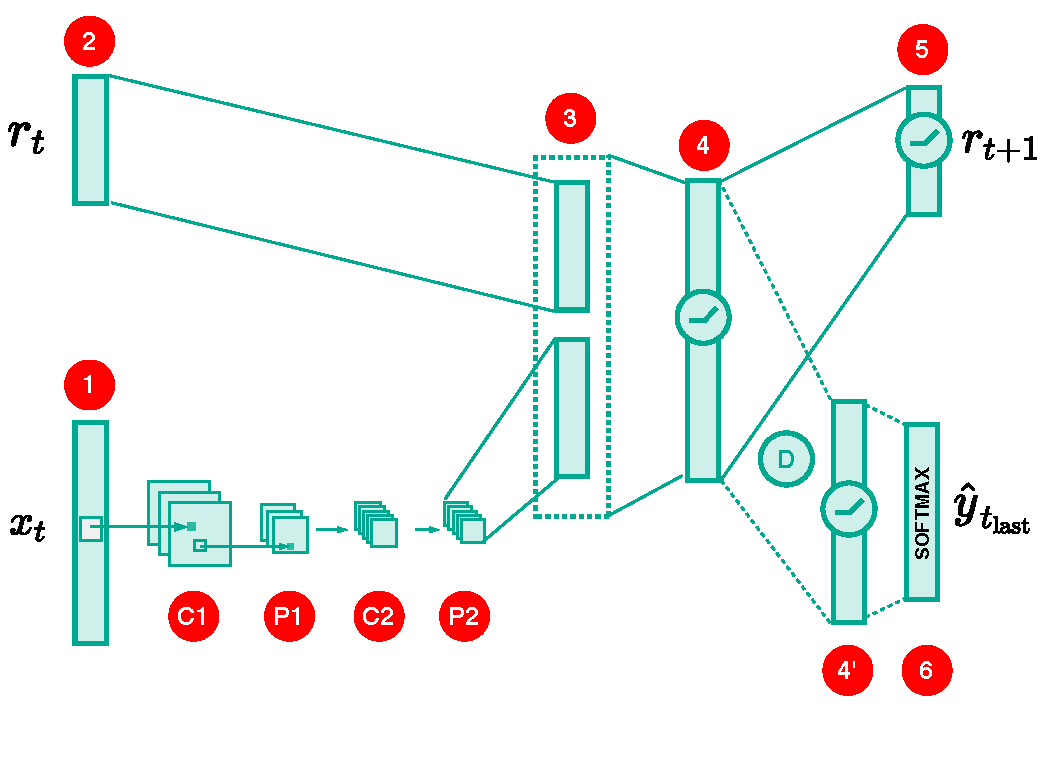
\includegraphics[width=0.6\textwidth]{sketch/convdeep_4l_network}
%\caption{ConvDeep Architecture}
%\label{fig:convdeep_4l_network}
%\end{figure}

Two variations of \rnncell{Deep} cell are also experimented, namely \rnncell{DeepV2} and \rnncell{ConvDeep}, shown on \addfigure{\ref{fig:deep_conv_arch}}. The former has one additional layer \circled{1"} with dropout regularization  between \circled{1'}. On the other hand, the latter replaces fully connected layers between \circled{1} and \circled{3} with 2 convolutional and max pooling layers, \Big[\circled{C1}, \circled{P1}\Big] and \Big[\circled{C2},\circled{P2}\Big].




\section{Setup}\label{sec:setup}
 
 I implemented experiments using TensorFlow\footnote{\url{http://tensorflow.org/}}.  weights $w_{ij} \in \patmatrix{W}$ and biases $b_{j} \in \patvector{b}$ are initialized as follows:
\begin{align*}
	w_{ij} &\sim \Psi( \mu=0, \sigma =0.1, [-2\sigma, 2\sigma]) \\
	b_{j} &= \ln(e^{0.01} - 1)
\end{align*}
where $\Psi(\cdot)$ denotes Truncated Normal Distribution with valid region between $[-2\sigma, 2\sigma]$.

%TODO : Figure normal distribution vs trucated

Activations $\patvector{a}^{(l)}_\cdot$ of layer $l$ is calculated using :
\begin{align*}
	\patvector{h}^{(l)}  &=  	\patmatrix{W}^T \patvector{a}^{(l-1)} - \sigma_{s}(\patvector{b}) \\
	\patvector{a}^{(l)}  &=  	\sigma_{r} (	\patvector{h}^{(l)} )
\end{align*}

where
\begin{align*}
	\sigma_{r} (h_j) &= \max(0, h_j)  \tag{ReLU function}\\
	\sigma_{s} (b_j) &= \log(1+\exp b_j) \tag{Softplus function}
\end{align*}
%TODO : Figure softplus vs relu

The reason of using $\sigma_{s} (b_j)$ for bias term is due to the non positive bias assumption of DTD. Moreover, $\sigma'_{s} (b_j)$ is $(0, \infty)$, as a result the network has more flexibility to adjust decision through back-propagation rather than using $\sigma_{r} (b_j)$. With this setting, the initial value of bias term  $\sigma_{s}(b_j)$ is then 0.01.

Speaking about training methodology, I use Adam\cite{KingmaAdamMethodStochastic2014} optimizer to train networks. Preliminary study shows that relevance heatmaps from networks trained by Adam are less noisy than the ones from other optimizers, such as  Stochastic Gradient Descent(SGD). Number of epochs is set to 200, while dropout probability is 0.5 and batch size is 50.  
Learning rate is not fixed as it is likely that different network architectures requires different value to achieve good performance, hence left adjustable. Table \ref{tab:hyper_summary} summaries the setting of hyperparameters.

%TODO: Figure Heatmaps SGD, RMSProp, Adam
 
 \begin{table}[!htb]
\centering
\begin{tabular}{l|r}
\textbf{Hyperparameter} & \multicolumn{1}{l}{\textbf{Value}} \\ \hline
Optimizer               & Adam                               \\
Epoch     & 200                                \\
Dropout Probability     & 0.5                                \\
Batch size              & 50                                
\end{tabular}
\caption{Hyperparameter Summary}
\label{tab:hyper_summary}
\end{table}
 
Traditionally, number of neurons in each layer ($n^{(l)}$) is  another hyperparameter that we can adjust. However, as the goal is to compare relevance heatmaps from different architectures, those numbers are fixed and chosen in such a way that total number of variables in each architecture are equivalent. \addfigure{\ref{fig:neuron_numbers}} illustrates the details of the settings.

\begin{figure}[!htb]
\centering
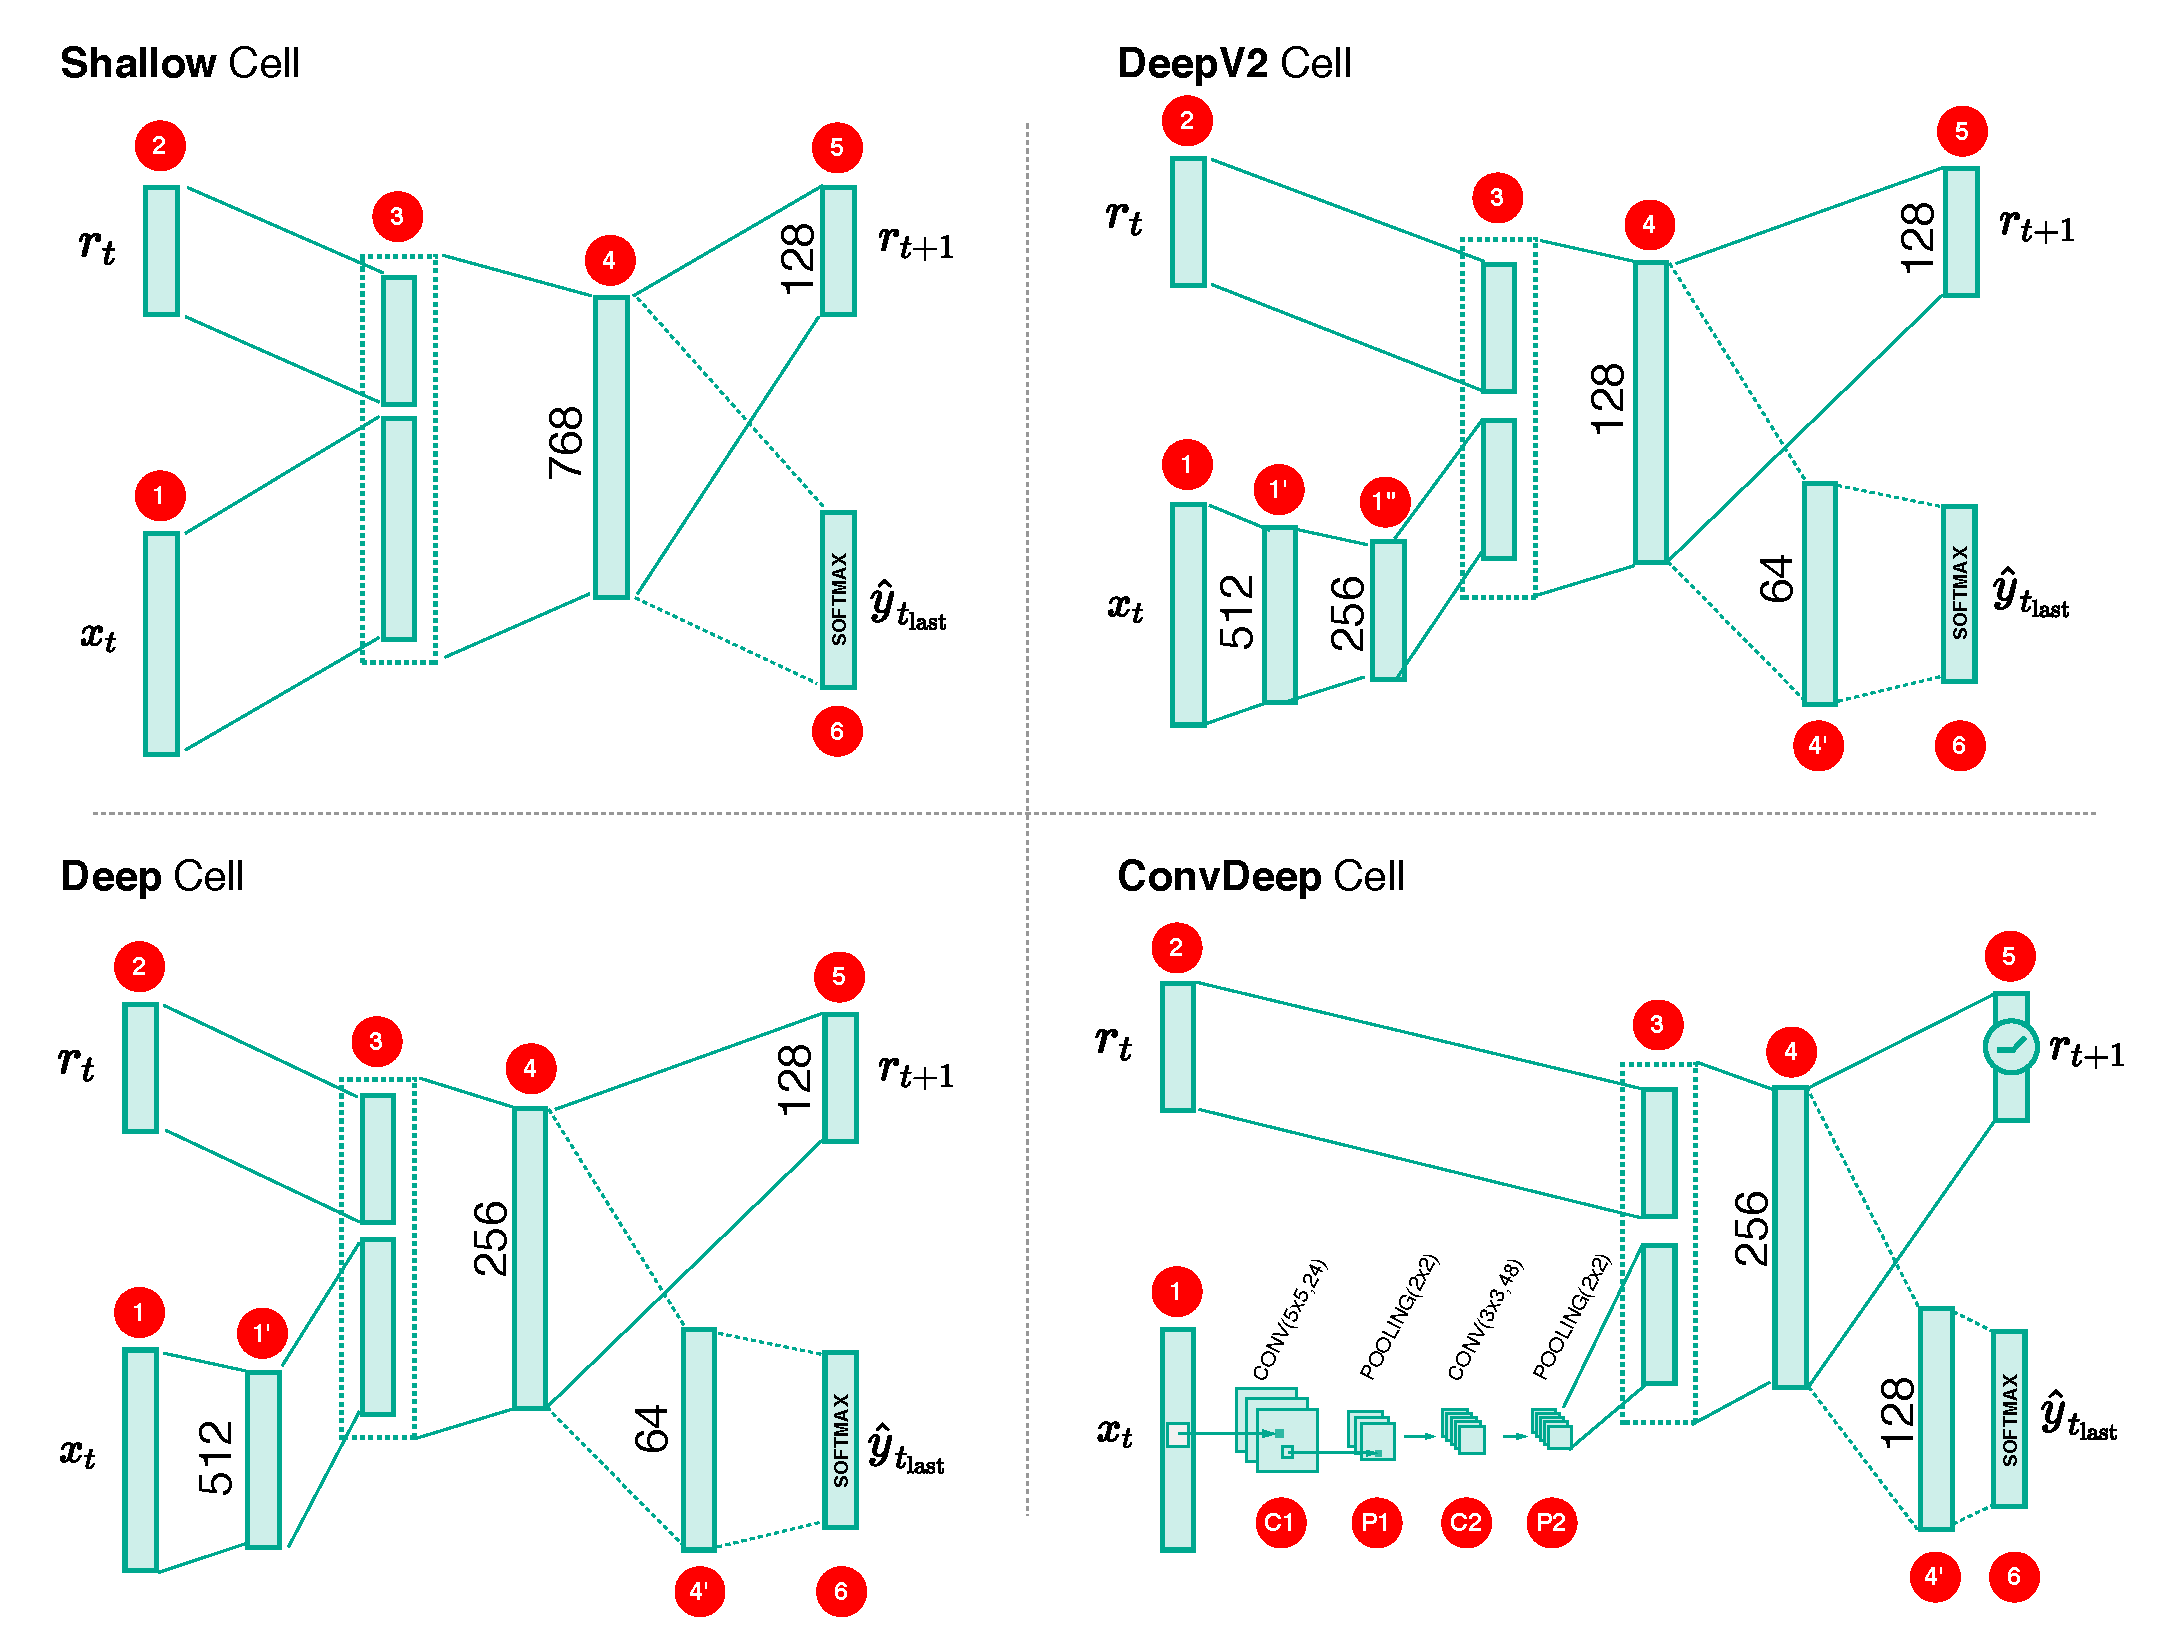
\includegraphics[width=\textwidth]{sketch/neuron_numbers}
\caption{Number of neurons in each layer for each cell architecture}
\label{fig:neuron_numbers}
\end{figure}


\begin{itemize}
	\item \textbf{Shallow Cell} 
$$\{ n^{(4)}\} = \{ 768 \}$$
	\item \textbf{Deep Cell} 
$$\{ n^{(1')}, n^{(4)}, n^{(4')} \} = \{ 512, 256, 64 \}$$
	\item \textbf{DeepV2 Cell} 
$$\{ n^{(1')}, n^{(1")}, n^{(4)}, n^{(4')} \} = \{ 512, 256, 128, 64 \}$$
	\item \textbf{ConvDeep Cell} : 
\begin{align*}
	\{ n^{(C1)}, n^{(P1)} \} &= \{ CONV(5\text{x}5, 24), POOL(2\text{x}2) \} \\
		\{ n^{(C2)}, n^{(P2)} \} &= \{ CONV(3\text{x}3, 48), POOL(2\text{x}2) \} \\
			\{  n^{(4)}, n^{(4')} \} &= \{ 256, 128 \}
\end{align*}
where $CONV(x,y)$ is a convolutional operator with $y$ filters whose kernel size is $\mathbb{R}^{x}$. Similarly, $POOL(x)$ is a pooling operator  with kernel size $\mathbb{R}^{x}$.


\end{itemize}

Noting that, $n^{(5)}$ is set at 128 for all architectures and 0 when the sequence length of the problem is 1. $n^{(6)}$ is equal to the number of categories of a problem, for example $n^{(6)} = 10 $ MNIST. Table \ref{tab:variable_architecture} shows the total numbers of variables in details.

\renewcommand{\arraystretch}{1.2}
\begin{table}[h]
\centering
\begin{tabular}{l|c|c|c|c|}
\cline{2-5}
                                                 & \multicolumn{4}{c|}{\textbf{Sequence Length}} \\ \hline
\multicolumn{1}{|l|}{\textbf{Cell Architecture}} & 1         & 4         & 7         & 14        \\ \hline
\multicolumn{1}{|l|}{\rnncell{Shallow}}                    & 610570    & 355722    & 291210    & 248202    \\ \hline
\multicolumn{1}{|l|}{\rnncell{Deep}}                       & 550346    & 314954    & 271946    & 243274    \\ \hline
\multicolumn{1}{|l|}{\rnncell{DeepV2}}                    & 575050    & 306890    & 263882    & 235210    \\ \hline
\multicolumn{1}{|l|}{\rnncell{ConvDeep}}                   & 647594    & 283178    & 197162    & 197162    \\ \hline
\end{tabular}
\caption{Total variables in each architecture and sequence length}
\label{tab:variable_architecture}
\end{table}


Lastly, as the quality of relevance heatmap depending on performance of the model, the minimum classification accuracy is set as in Table  \ref{tab:min_acc}. 

\begin{table}[h]
\centering
\begin{tabular}{ll}
\multicolumn{1}{l|}{\textbf{Dataset}} & \textbf{Minimum Accuracy} \\ \hline
\multicolumn{1}{l|}{MNIST}            & \multicolumn{1}{r}{0.98}  \\
\multicolumn{1}{l|}{Fashion-MNIST}    & \multicolumn{1}{r}{0.85}  \\
%\multicolumn{1}{l|}{UFI Cropped}                                       &                         \dots
\end{tabular}
\caption{Classification Accuracy Criteria}
\label{tab:min_acc}
\end{table}


\section{Experiment 1 : Sequence Classification}

\subsection{Problem Formulation}
To demonstrate how well RNNs can distribute relevant quantities to input space, I formulated an artificial classification problem in which each image sample $\x$ is column-wise split into non-overlapping $(\x_t)_{t=1}^{T}$.  The RNN classifier needs to summarize information from the sequence $(\x_t)_{t=1}^{T}$ to answer what is the class of $\x$.   

\addfigure{\ref{fig:artificial_problem}} illustrates the setting. Here, a MNIST sample $ \patvector{x} \in \mathbb{R}^{28,28}$ is divided to a sequence of $( \patvector{x}_t \in   \mathbb{R}^{28,7} )_{t=1} ^ 4$. At time step $t$, $\patvector{x}_t$ is presented to the RNN classifier which yields recurrent input $\patvector{r}_{t+1}$ for the next step. For the last step $T$, in this example $T = 4$, the RNN classifier computes $f(\x) \in \mathbb{R}^{10}$ and the class that $\x$ belongs to. 

 \begin{figure}[!hbt]
\centering
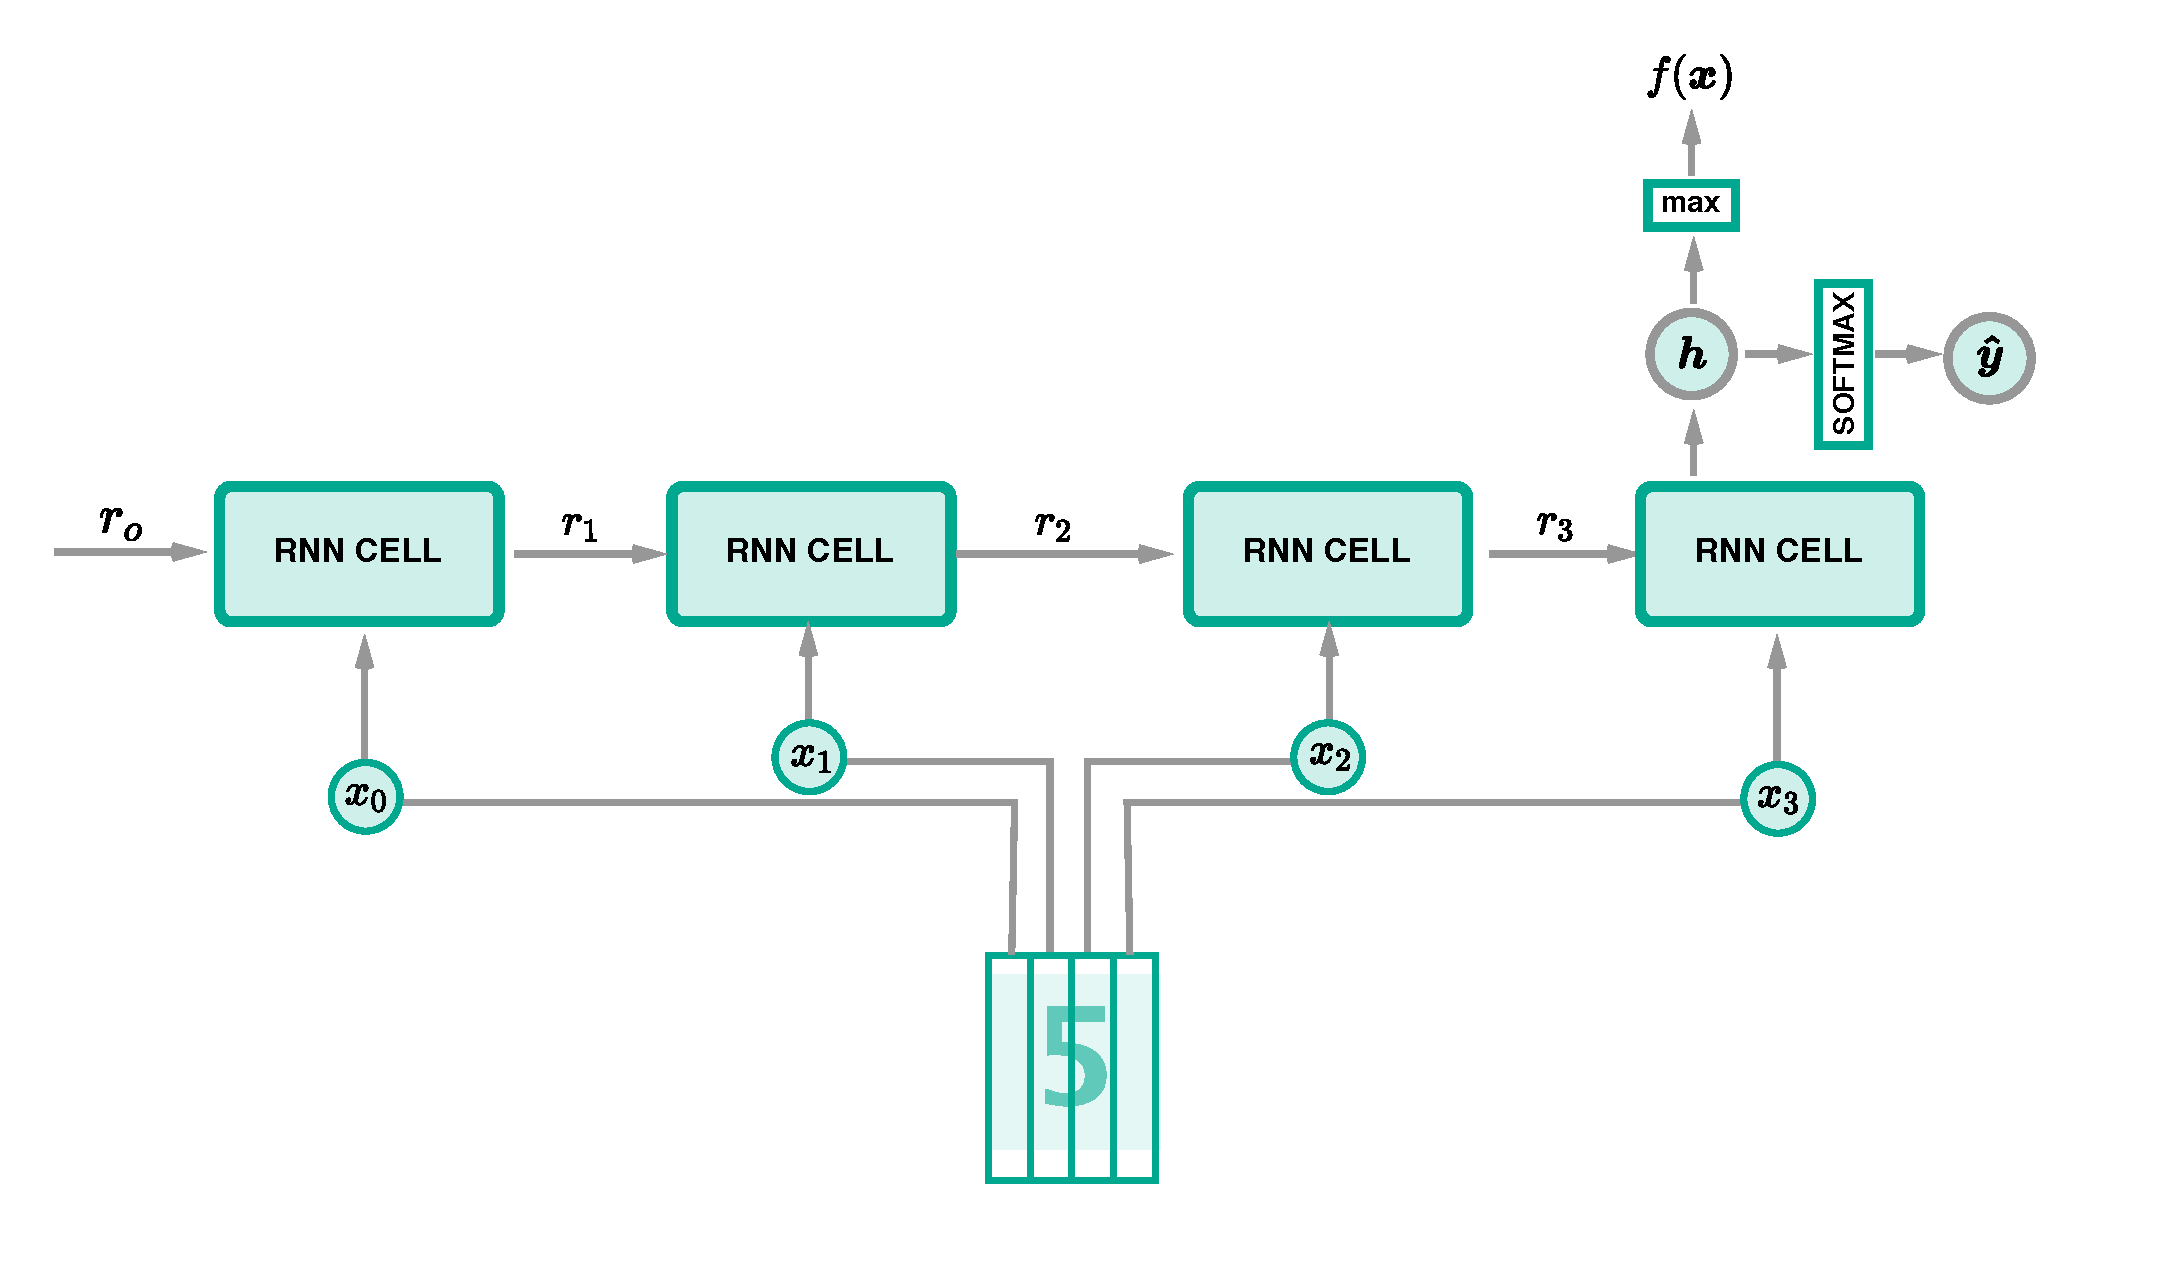
\includegraphics[width=0.9\textwidth]{sketch/artificial_problem}
\caption{General setting of RNN classifiers in this thesis} 
\label{fig:artificial_problem}
\end{figure}

 Denote $g_r$ and $g_{f}$ function that the RNN  with parameters $\boldsymbol{\theta}$ uses to compute $\patvector{r}_{t+1}$ and $f(\x)$ respectively. The overall computation can be summarized as follows: 
 \begin{align*}
 	\patvector{r}_{t+1} &= g_r(\patvector{\theta}, \patvector{x_t}, \patvector{r_t}) \\
 	 &\ \ \vdots\\
f(\x) &= g_{h}(\patvector{\theta}, \patvector{x}_{t_{\text{last}}},  \patvector{r}_{t_{\text{last}}}) \\
 	\patvector{\hat{y}} &= \text{softmax}(f(\x)),
 \end{align*}
 where $\patvector{\hat{y}}$ is the class probabilities and $\patvector{r}_0 = \patvector{0}$.   To explain the model,  $R(\x)$ is set to the value of $f(\x)$ that is corresponding to the true target class.
 
 \todo{Figure figure show how R(x) is set?}
 
 
\renewcommand{\arraystretch}{1.5}
\begin{table}[h]
\centering
\begin{tabular}{l|l|l|l|l|}
\cline{2-4}
                                            & \multicolumn{3}{c|}{Sequence Length}                                                               \\ \hline
\multicolumn{1}{|c|}{Dataset}               & \multicolumn{1}{c|}{1} & \multicolumn{1}{c|}{4} & \multicolumn{1}{c|}{7}  \\ \hline
\multicolumn{1}{|l|}{MNIST / FashionMNIST} &        $ \mathbb{R}^{28,28}  $              &          $ \mathbb{R}^{28,7}  $               &         $ \mathbb{R}^{28,4}  $                            \\ \hline
%\multicolumn{1}{|l|}{UFI-Cropped}           &                        &                        &                        &                         \\ \hline
%\multicolumn{1}{|l|}{}                      &                        &                        &                        &                         \\ \hline
\end{tabular}
\caption{Dimensions of $\patvector{x}_t$ for each dataset and sequence length}
\label{tab:seq-length}

\end{table}
\renewcommand{\arraystretch}{1}

%In this section, I am going to present what I have  found from experiments. First, I am going to discuss results from MNIST and then move on to ones from Fashion-MNIST. Moreover, I will use \rnncellseq{CELL\_NAME}{SEQ} convention to denote a RNN network with CELL\_NAME cell trained on a sequence length SEQ. For example, \rnncellseq{Deep}{7} means a RNN with Deep cell architecture trained on data whose $\patvector{x}^{(\alpha)}$ is a sequence of length 7.


\subsection{Result}
I began this preliminary experiment  with Shallow and Deep architecture. They were trained on MNIST and FashionMNIST with sequence length $T = \{1, 4, 7\}$. Table \ref{tab:seq-length} shows dimensions of $\patvector{x}_t$ for different sequence length and Table \ref{tab:mnist_model_acc} summaries accuracy of the trained models. To simplify the manuscript, I am going to use \textit{\rnncellseq{ARCHITECTURE}{T}} convention to denote a RNN with \textit{ARCHITECTURE} trained on sequence length \textit{T}. For example, \rnncellseq{Deep}{7} refers to the Deep RNN architecture trained on $(\x_t \in \mathbb{R}^{28,4} )_{t=1}^{7}$.


\begin{table}[]
\centering
\begin{tabular}{lrr}
\textbf{}                  & \multicolumn{1}{c}{\textbf{Shallow}} & \multicolumn{1}{c}{\textbf{Deep}} \\ \hline
\multicolumn{1}{l|}{SEQ-1} & xx.xx\%                              & xx.xx\%                           \\
\multicolumn{1}{l|}{SEQ-4} & xx.xx\%                              & xx.xx\%                            \\
\multicolumn{1}{l|}{SEQ-7} & xx.xx\%                              & xx.xx\%
\end{tabular}
\caption{Model Accuracy}
\label{tab:mnist_model_acc}
\end{table}


 \begin{figure}[h]
\centering
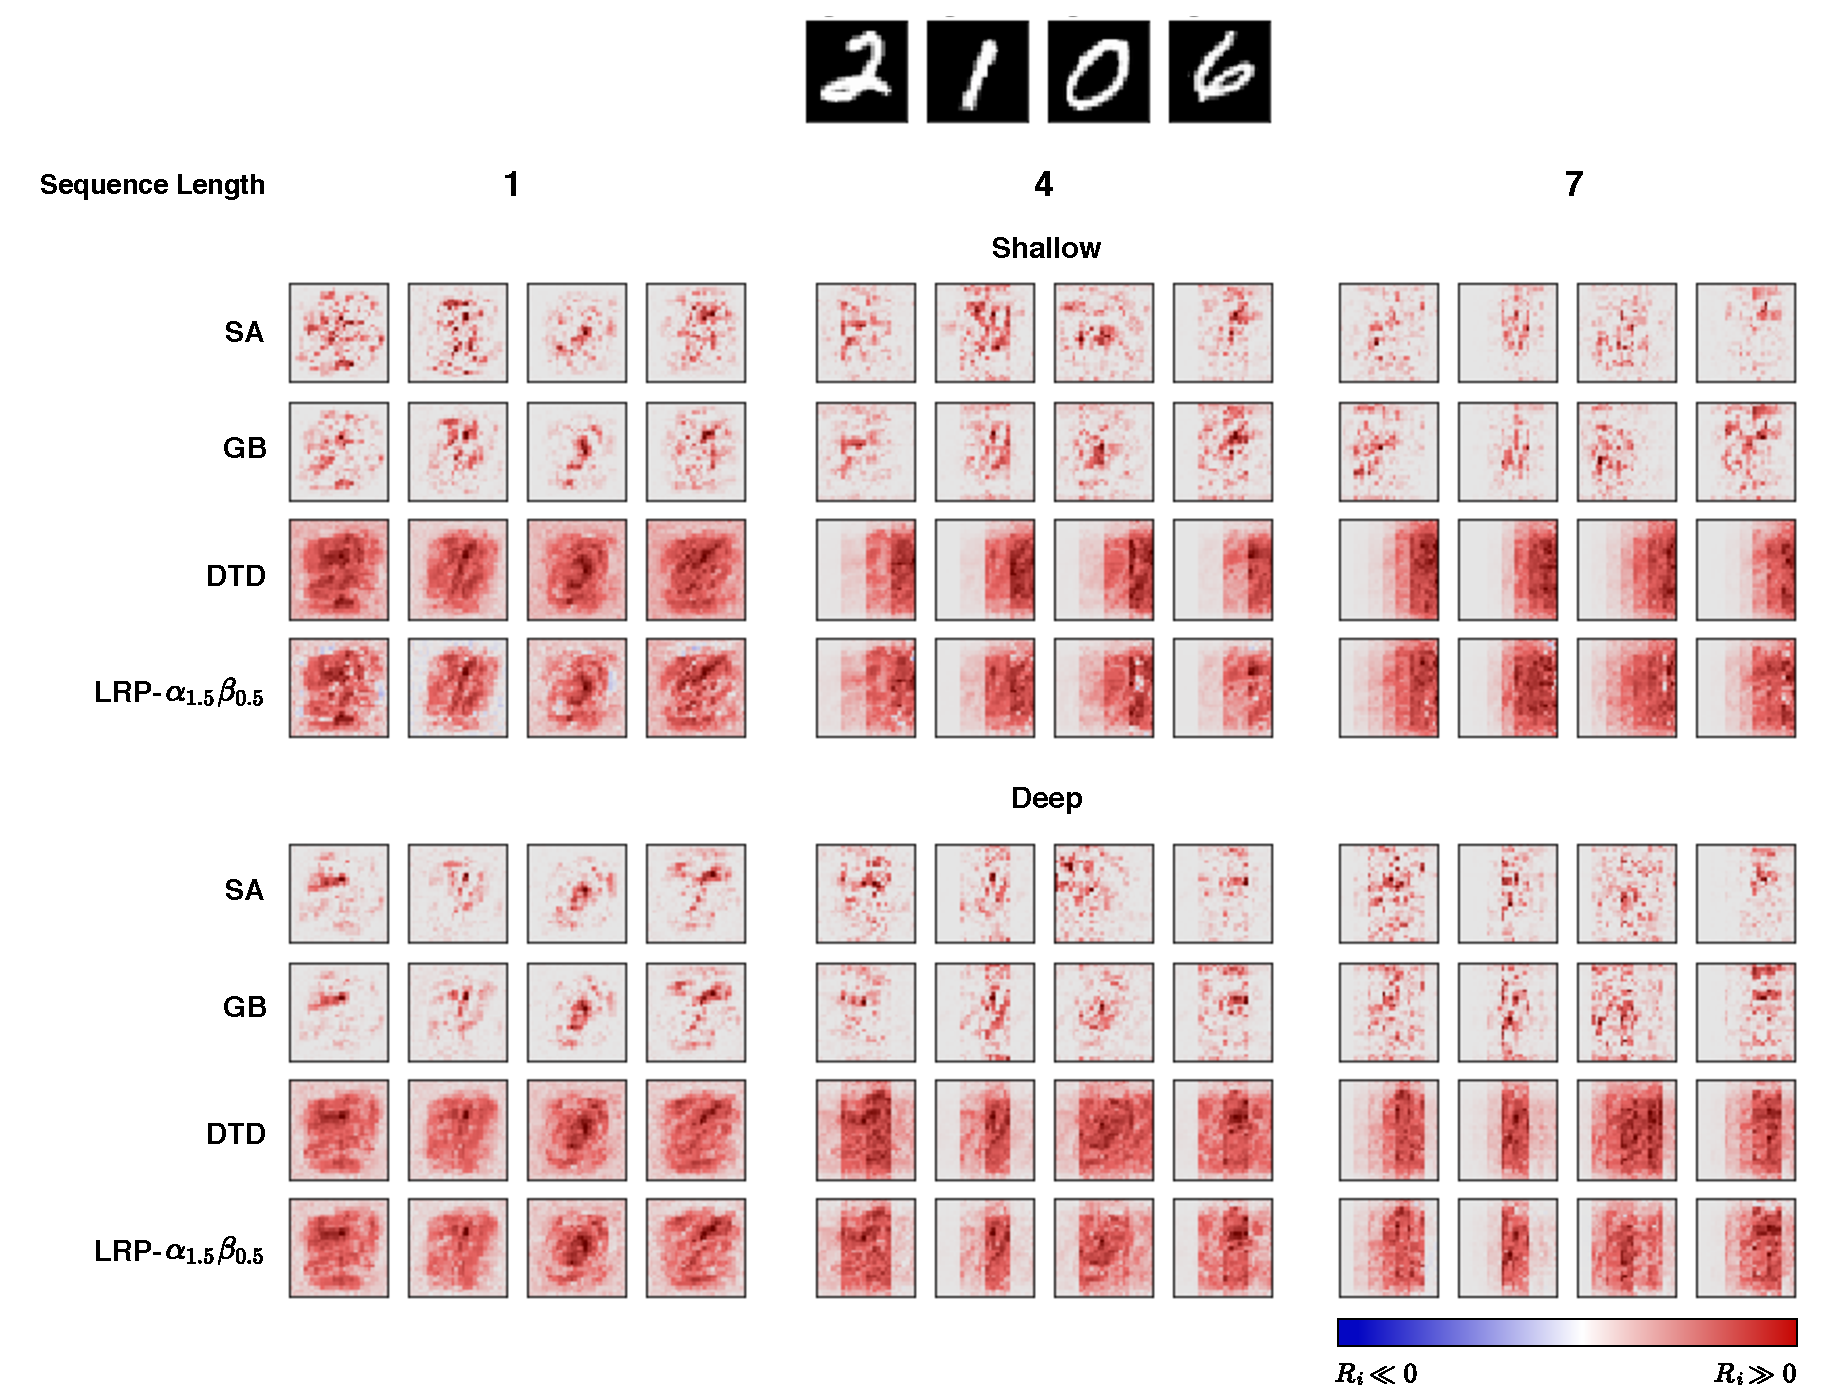
\includegraphics[width=0.8\textwidth]{sketch/mnist_experiment}
\caption{Relevance heatmaps from Shallow and Deep Cell trained on MNIST with different sequence lengths}
\label{fig:mnist_experiment}
\end{figure}


\addfigure{\ref{fig:mnist_experiment}} shows relevance heatmaps from Shallow and Deep architecture trained on MNIST.  We can see general characteristics of each explanation technique. In particular, sensitivity analysis(SA) and guided backprop(GB) heatmaps are sparse, while the ones from deep Taylor decomposition(DTD) are more diffuse throughout $\x$.  When applying these techniques to \rnncellseq{Shallow}{1}  and \rnncellseq{Deep}{1}, the relevance heatmaps look similar regardless of the architectures.  As the sequence length is increased, SA and GB heatmaps are still almost identical  for \rnncellseq{Shallow}{4,7} and \rnncellseq{Deep}{4,7}. However, this is not the case for DTD.  From the figure, we can see that \rnncellseq{Shallow}{4,7} and  \rnncellseq{Deep}{4,7} return significantly different relevance heatmaps from DTD method.  In particular,  \rnncellseq{Shallow}{4,7} 's heatmaps are mainly concentrated on the right part of $\x$ associating to last time steps, while  \rnncellseq{Deep}{4,7}'s ones are appropriately highlighted at the actual content area of $\x$.


 \begin{figure}[h]
\centering
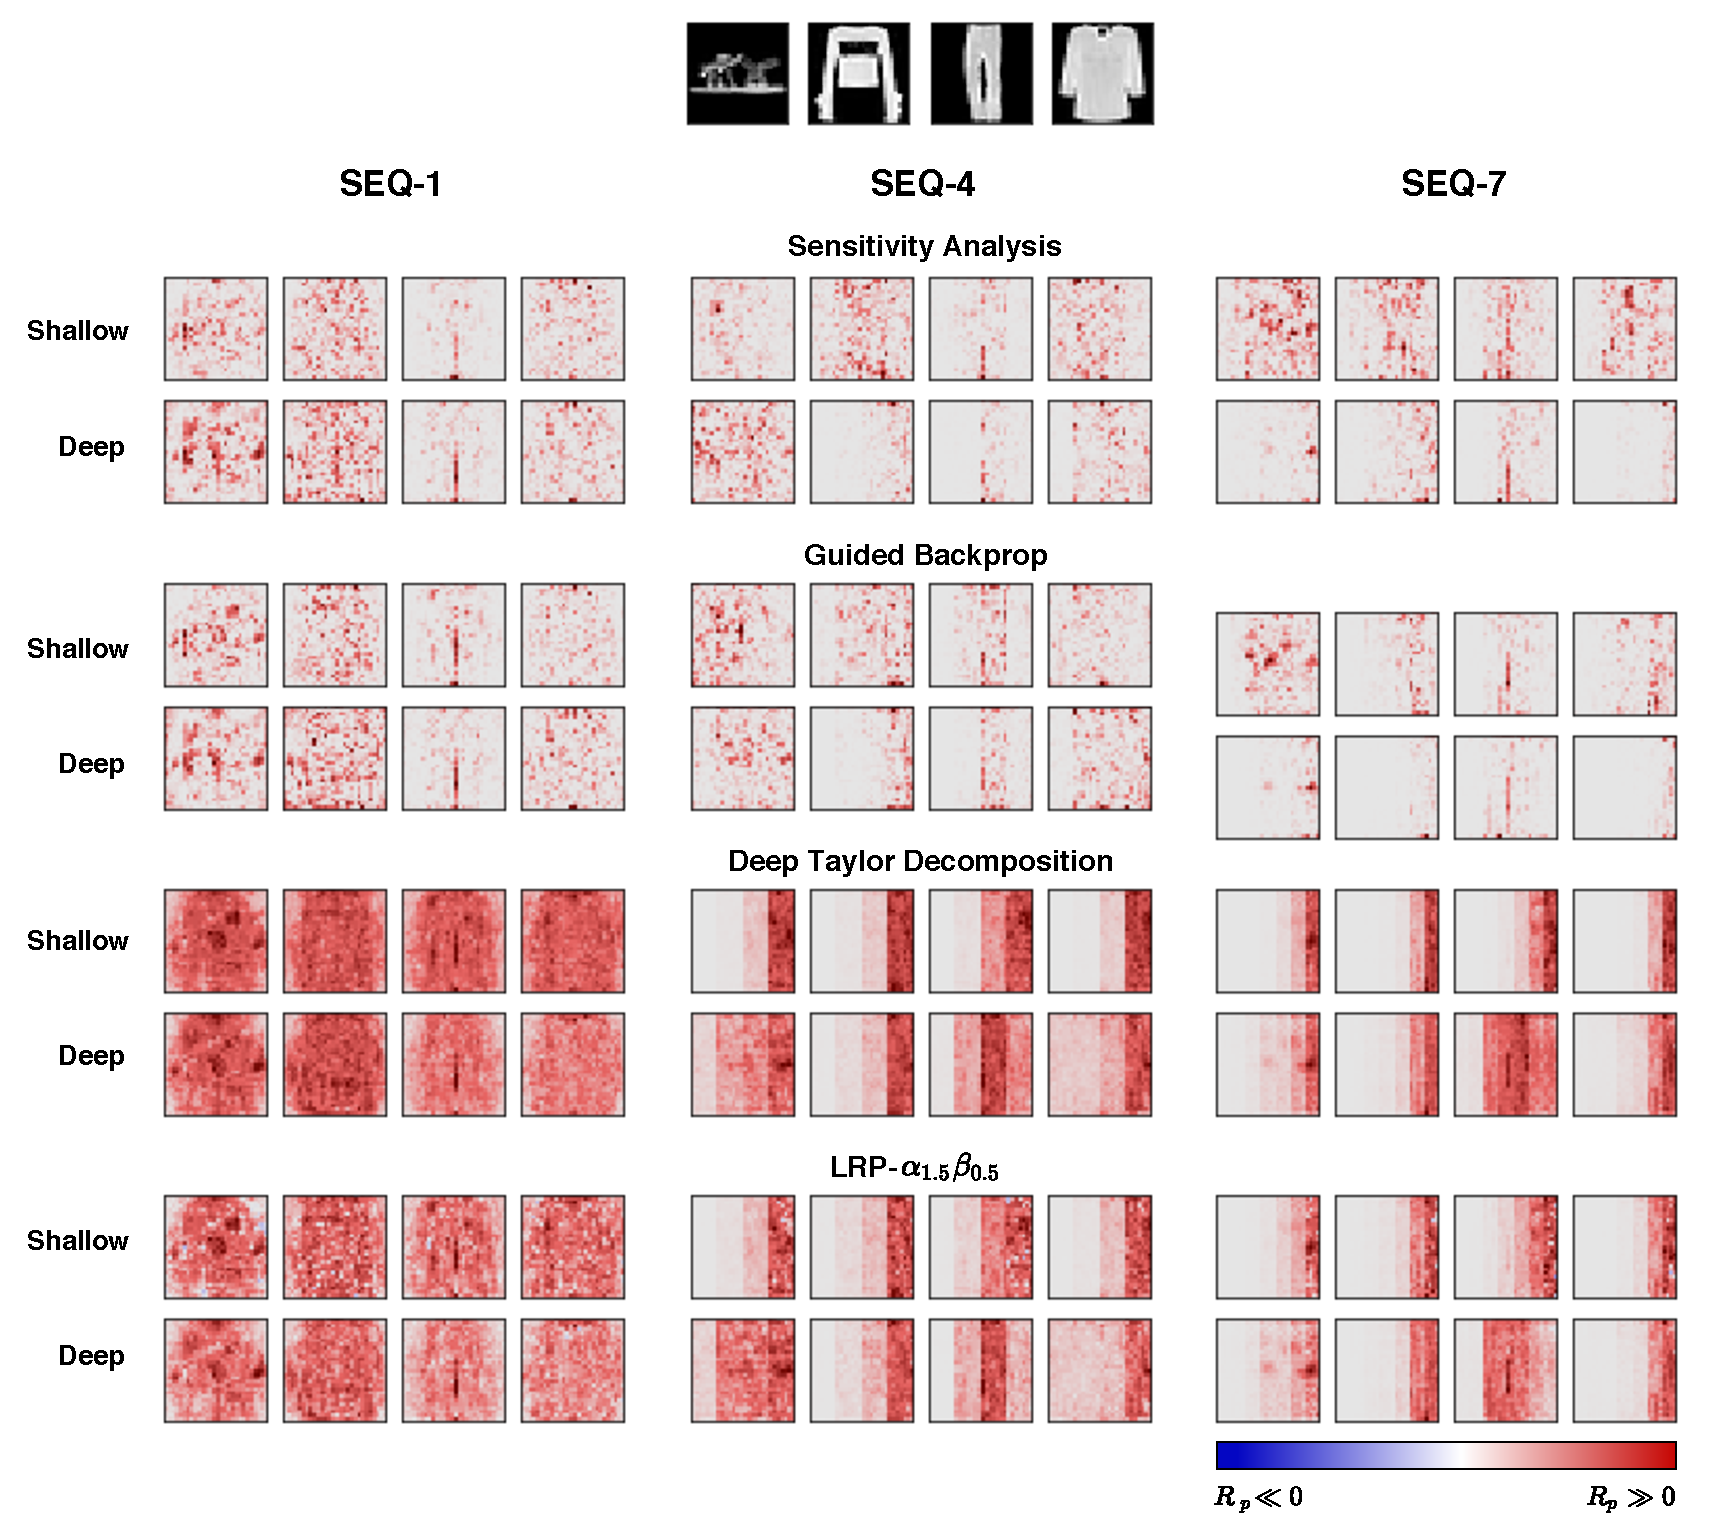
\includegraphics[width=0.8\textwidth]{sketch/fashion_mnist_experiment}
\caption{Relevance heatmaps from Shallow and Deep Cell trained on FashionMNIST with different sequence lengths}
\label{fig:fashion_mnist_experiment}
\end{figure}

Relevance heatmaps of Shallow and Deep architecture trained on  FashionMNIST  are shown on \addfigure{\ref{fig:fashion_mnist_experiment}}. Similar to MNIST, we do not see any remarkable difference on SA and GB heatmaps of the two architectures : only that \rnncellseq{Deep}{4,7} produces slightly more sparse heatmaps. Although the wrong concentration issue of DTD  seems to appear on both \rnncellseq{Shallow}{4,7}'s and \rnncellseq{Deep}{4,7}'s heatmaps, we still can observe proper highlight from Deep architecture on some samples. For example, the trouser sample, we can see  that \rnncellseq{Deep}{4,7} architecture manage to distribute high relevance scores to area of the trouser. Latent features of FashionMNIST  might be one of the reasons why Deep architecture does not distribute relevance scores to early steps for the FashionMNIST samples. Consider \textit{Shoe} and \textit{Ankle Boot} samples in \addfigure{\ref{fig:fashion_mnist_samples}}. One can see that  their front part are similar and only the heel part that determines the differences between the two categories.




 \begin{figure}[ht!]
\centering
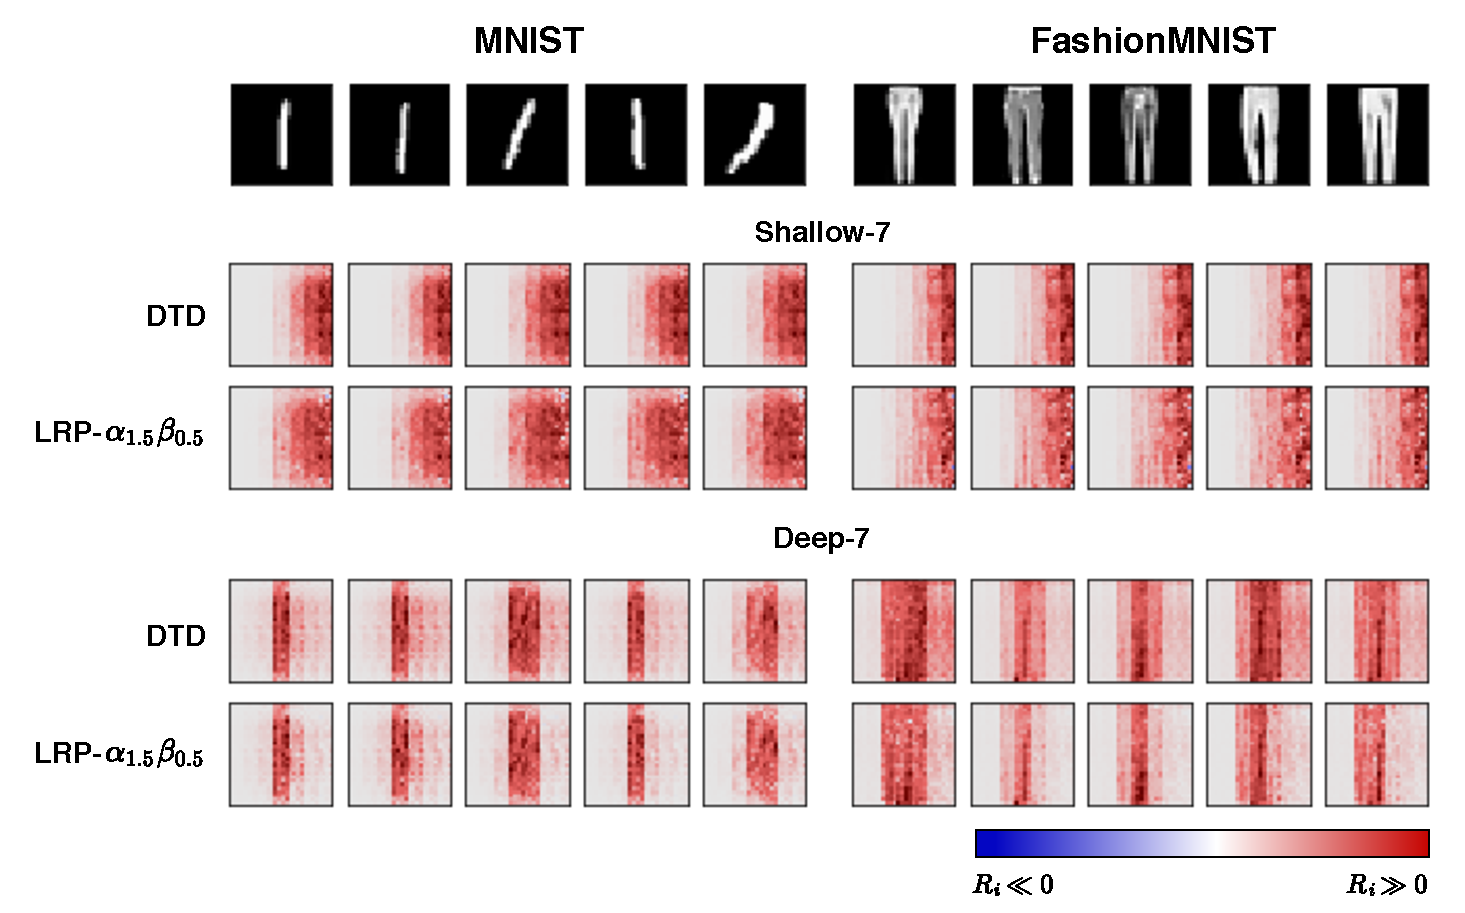
\includegraphics[width=\textwidth]{sketch/class_1_comparison}
\caption{DTD relevance heatmaps of MNIST \textit{Class 1} and FashionMNIST \textit{Class Trouser} samples from \rnncellseq{Shallow}{7} and \rnncellseq{Deep}{7}. }
\label{fig:class_1_comparison}
\end{figure}

\addfigure{\ref{fig:class_1_comparison}} presents relevance heatmaps of MNIST \textit{Class 1} and FashionMNIST \textit{Class Trouser} samples. These samples were chosen to emphasize the impact of RNN architecture on DTD explanation. In particular,  these samples have $\x_{t'}$ containing features  primarily locating at the center, or middle of the sequence, hence appropriate relevance heatmaps should be highlighted at $\x_{t'}$ and possibly its neighbors.  As expected, we can see \rnncellseq{Deep}{7} produces sound results in which the  heatmaps have high intensity value where $\x_{t'}$ approximately locate, while \rnncellseq{Shallow}{7} mainly assigns relevance quantities to $\x_{t}$ for $t \approx T$. \addfigure{\ref{fig:exp1_dist_plot}} further shows a quantitive evidence of this problem. Here, distribution of relevance score from \rnncellseq{Shallow}{7} and \rnncellseq{Deep}{7} are plotted across time step $t = \{ 1, \dots, 7 \}$. The distributions are computed from all test samples in MNIST \textit{Class 1} and FashionMNIST \textit{Class Trouser} respectively as well as the data distributions that are derived from pixel intensity values.  We can see that \rnncellseq{Deep}{7}'s relevance distributions are similar to the data distributions, while  \rnncellseq{Shallow}{7}'s ones diverge completely. Particularly,  one can see that \rnncellseq{Shallow}{7} distributes more than 90\% of relevance scores to the last 3 steps, namely $\x_5$, $\x_6$ and $\x_7$.


 \begin{figure}[h]
\centering
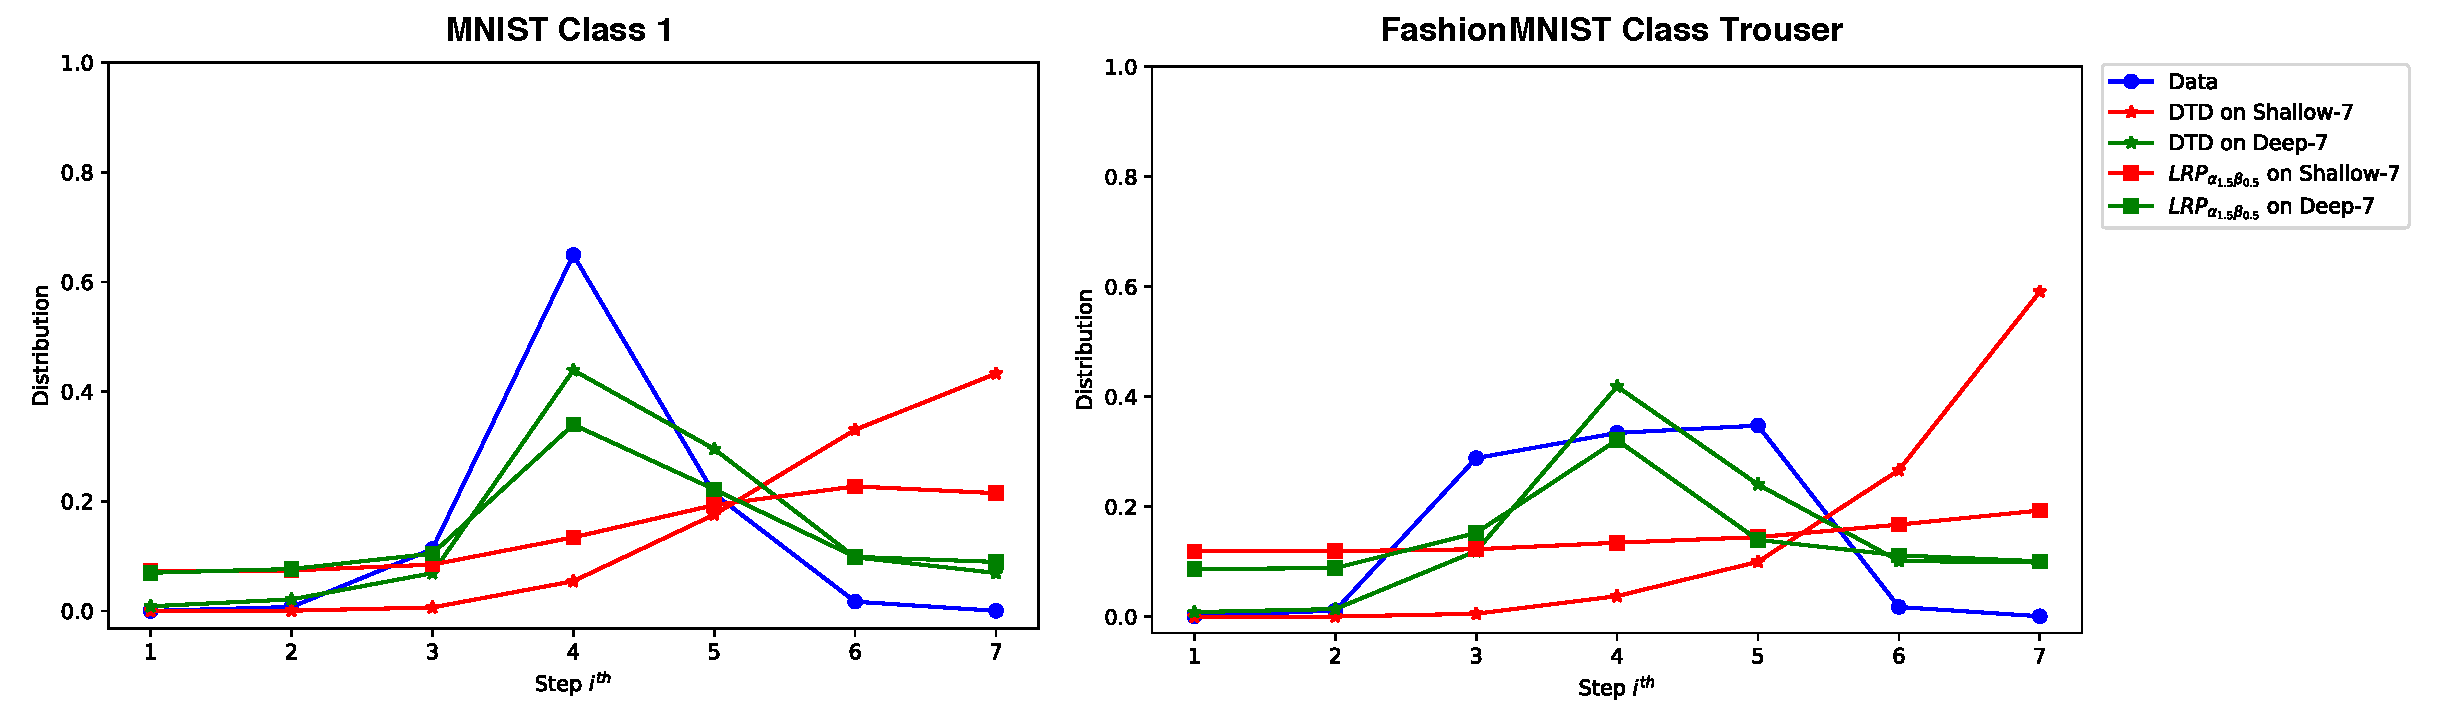
\includegraphics[width=\textwidth]{sketch/exp1_dist_plot}
\caption{Pixel intensity and DTD relevance distribution from \rnncellseq{Shallow}{7} and \rnncellseq{Deep}{7} averaged over MNIST \textit{Class 1} and FashionMNIST \textit{Class Trouser} test population.} 
\label{fig:exp1_dist_plot}
\end{figure}

\subsection{Summary}
Results from this first experiment seem to suggest that choice of RNN architectures has an impact on quality of its explanation.  In particular,  as presented in \addfigure{\ref{fig:class_1_comparison}} and \addfigure{\ref{fig:exp1_dist_plot}}, quality of deep Taylor decomposition(DTD) explanation is significantly influenced by the architecture. In contrast, we do see such notable effect from sensitivity analysis(SA) and guided backprop(GB) method.  In the following experiment, I am going to present a methodical evaluation of this impact in detail.



\section{Experiment 2 : Majority Sample Classification} \label{sec:exp2}
   
 \begin{figure}[h]
\centering
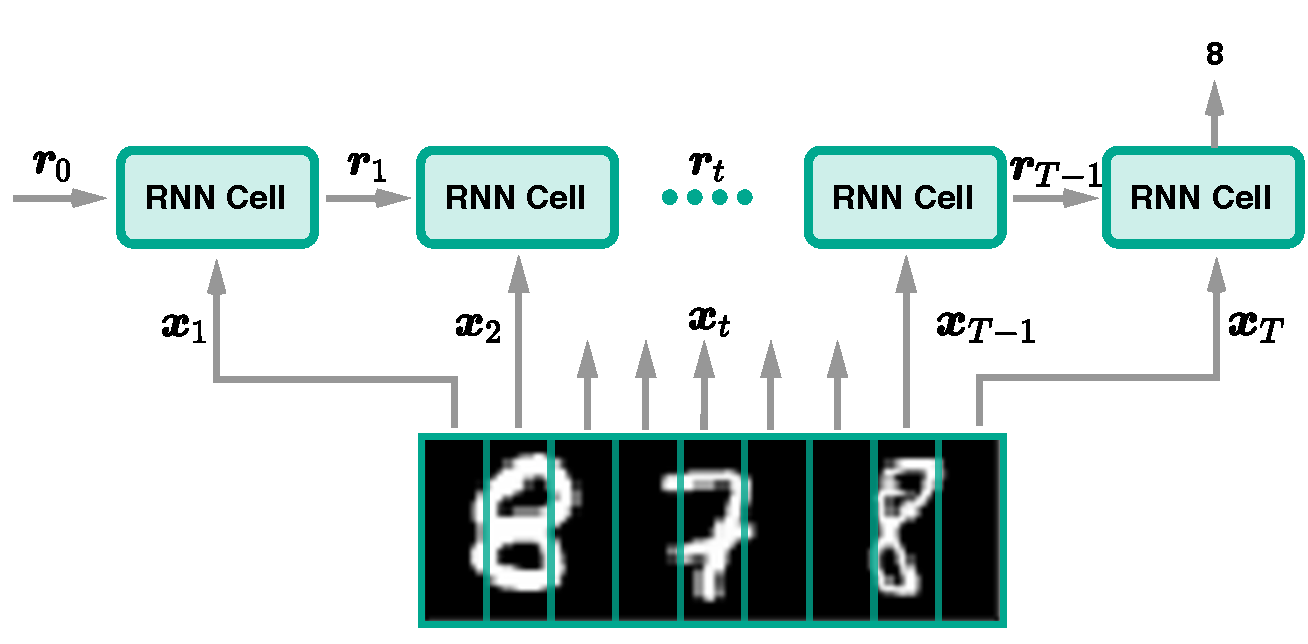
\includegraphics[width=0.7\textwidth]{sketch/artificial_problem_3digits}
\caption{Majority Sample Classification Problem} 
\label{fig:artificial_problem_3digits}
\end{figure}

\subsection{Problem Formulation} \label{sec:exp2_prob_formulate}
When neural network are trained, one can apply explantation techniques to the models to get relevance heatmaps of samples.  The heatmap of sample $\x$ illustrates important features in $x$ that the trained network utilizes to perform its objective prediction,  such as classification.  Therefore, one needs to know the ground truth of these latent features in order to methodologically evaluate how well the model distributes  relevance scores to $\x$'s input space. However,  this knowledge is not trivial to find as it is an incident from the optimization process in high-dimensional space that we in fact seek to understand.

To alleviate this challenge, I constructed two artificial datasets using samples from  MNIST and FashionMNIST respectively. Let's consider MNIST. The new dataset was constructed as follows: each original sample $\widetilde{\x} \in \mathbb{R}^{28,28}$, I randomly selected 2 additional samples : one from the same class of $\widetilde{\x}$ and the other one from a different class. Then, these 3 samples are concatenated in random order yielding a sample $\x \in \mathbb{R}^{28,84}$ of the new dataset. 

With this construction procedure, one possible objective  is to train RNNs to predict the majority class in each sequence $(\x_t )_{t=1}^{T}$. For example, consider $\x = \{ 8, 7, 8\}$ shown in \addfigure{\ref{fig:artificial_problem_3digits}}, the majority class here is \textit{Class 8}. Because we already know time step $t'$ that are corresponding to original samples $\widetilde{\x}$ belonging to the majority group in each sequence $\x$, we can simply compute percentage of relevance scores assigned to $t'$ to quantitively  evaluate explainability  of a RNN architecture. 

I also introduces two additional variation of Deep architecture, namely DeepV2 and ConvDeep. DeepV2 has one more layer after the first fully-connected layer, while ConvDeep instead employs a sequence of convolutional and pooling operation after the input layer. Figure X shows details of the architectures. 



 %Table x show accuracy sf

\subsection{Result}


\begin{table}[h]
\begin{center}
\begin{tabular}{l c|c|c|}
\cline{3-4}
& &
\multicolumn{2}{c|}{\parbox{3.5cm}{ \vskip 1mm \centering \textbf{Accuracy} \vskip 1mm}} \\ \hline
\multicolumn{1}{|l|}{\textbf{Cell Architecture}} & \textbf{No. variables} & \textbf{MNIST} & \textbf{FashionMNIST} \\ \hline
\multicolumn{1}{|l|}{Shallow}    & 184330                 & 98.39\% & 90.15\% \\ 
\multicolumn{1}{|l|}{Deep}       & 153578                 & 98.42\% & 90.60\% \\ 
 \multicolumn{1}{|l|}{DeepV2}     & 161386                 & 98.38\% & 90.43\% \\
\multicolumn{1}{|l|}{ConvDeep}   & 151802                 & 99.07\% & 92.43\%  \\ \hline 
\end{tabular}

\end{center}
\caption{Number of trainable variables and model accuracy for Majority Sample Classification experiment.}
\label{tab:maj_rnn_model_acc}
\end{table}

 \begin{figure}[h]
\centering
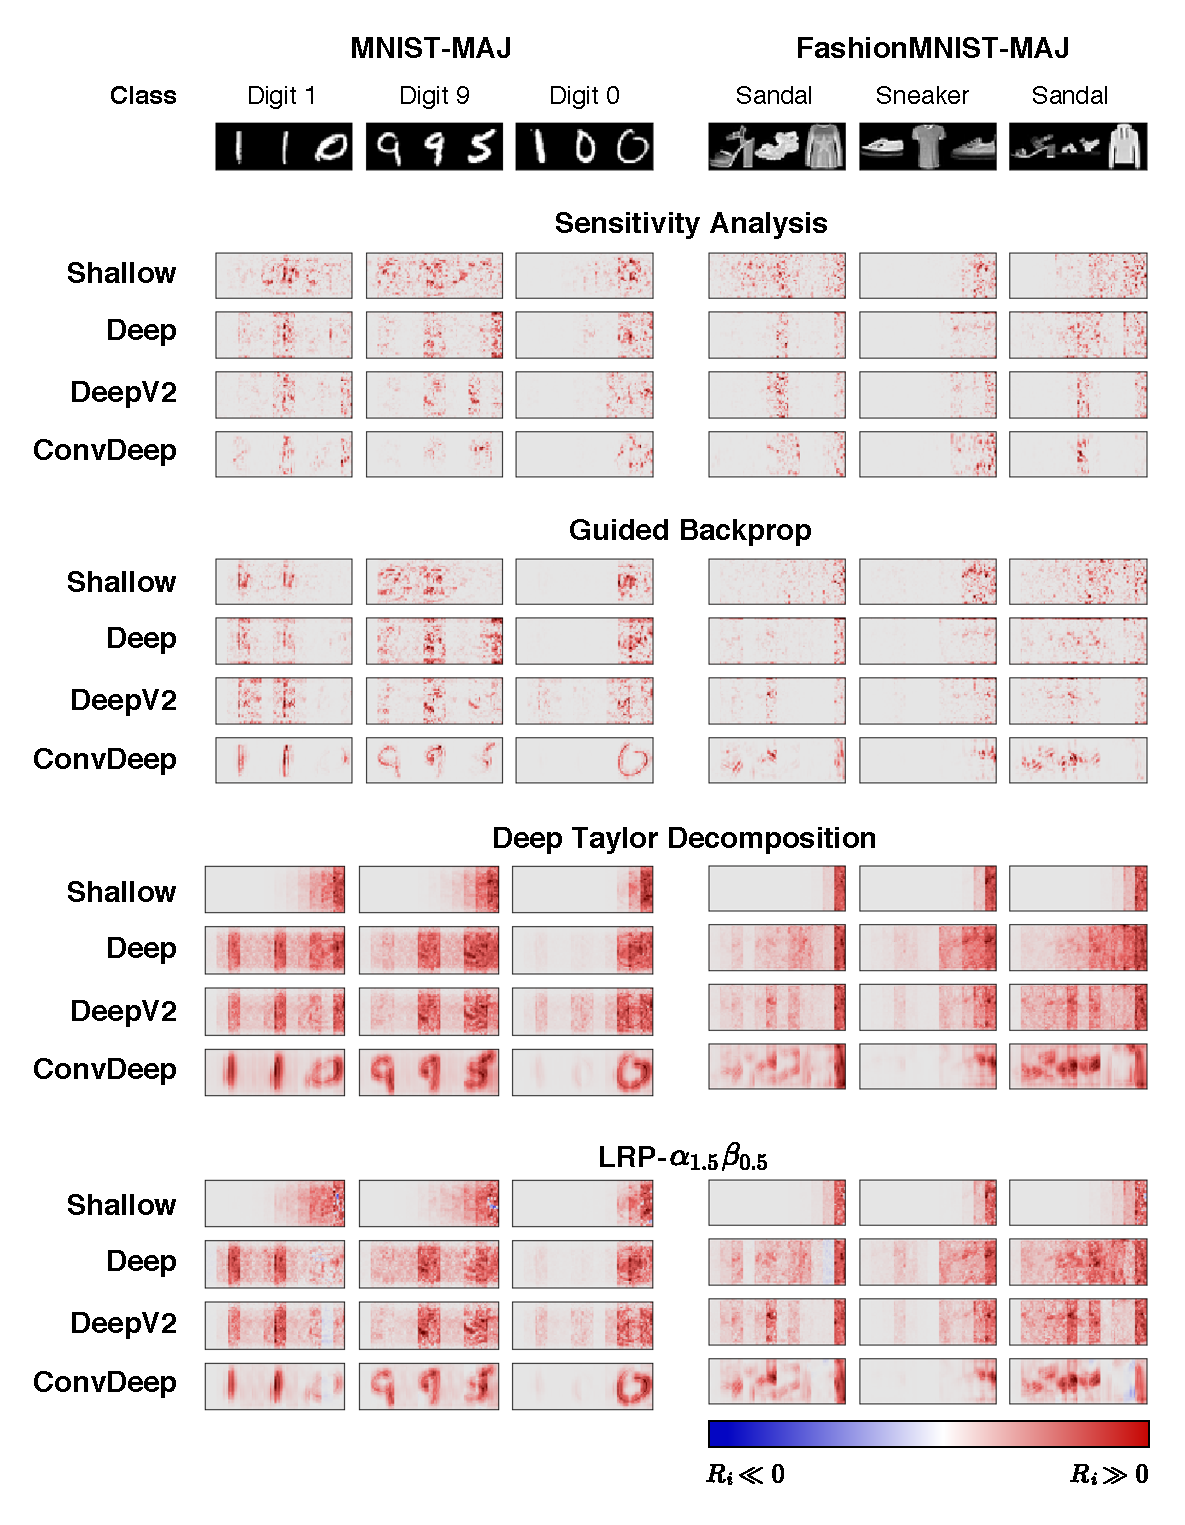
\includegraphics[width=\textwidth]{sketch/heatmap_msc_for_thesis}
\caption{Relevance heatmaps for MSC problem} 
\label{fig:heatmap_msc_mix_for_thesis}
\end{figure}

In this experiment, I chose $T=12$, hence $(\x_t \in \mathbb{R}^{28,7})_{t=1}^{12}$. Table \ref{tab:maj_rnn_model_acc} shows number of trainable variables and accuracy of the trained models. These trained models have equivalent number of variables and accuracy, hence comparing heatmaps of these models is a fair evaluation.

As can be seen from \addfigure{\ref{fig:heatmap_msc_mix_for_thesis}}, the deeper architecture, the fewer relevant scores distributed to irrelevant region. This effect happens across all explanation methods. This result further supports what has shown in Experiment 1.  Moreover, although relevance heatmaps from \rnncellseq{Shallow}{12}, \rnncellseq{Deep}{12}, and \rnncellseq{DeepV2}{12} generally look noisy, increasing the depth of architecture seems to reduce the noise in the heatmaps.   On the other hand, \rnncellseq{ConvDeep}{12} does not  only properly assign relevance quantities to the right time steps, but its heatmaps are also sound. In particular, one can easily perceive features of $\x$ from \rnncellseq{ConvDeep}{12}'s GB and DTD heatmaps.


 \begin{figure}[h]
\centering
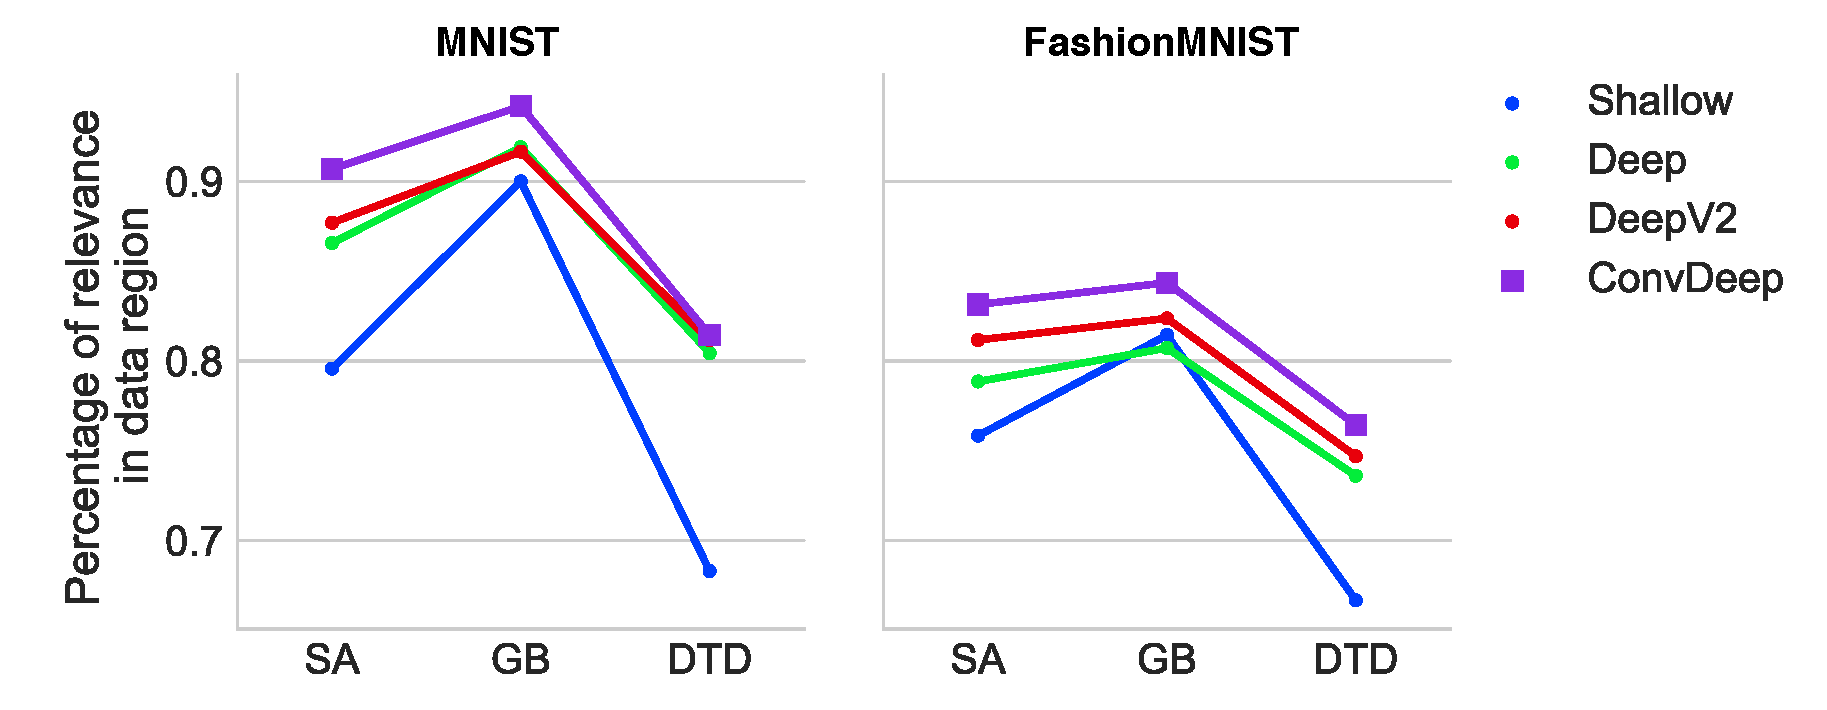
\includegraphics[width=0.7\textwidth]{sketch/rel_dist_maj_3_samples_thesis}
\caption{Percentage of relevance in data region} 
\label{fig:rel_dist_maj_3_samples_thesis}
\end{figure}

\addfigure{\ref{fig:rel_dist_maj_3_samples_thesis}} presents a quantitive  evaluation of the impact from the depth of architecture to the explanation. Here, the measurement is the percentage of relevance quantities assigned to regions of majority class : these regions are indicated by the red triangles in \addfigure{\ref{fig:heatmap_msc_mix_for_thesis}}, averaged over test sample population. Results from \addfigure{\ref{fig:rel_dist_maj_3_samples_thesis}} indicate that the depth of architecture indeed improves quality of the explanations. In particular, the percentage of correct relevance assignment of each explanation technique increases as more layers introduced. This enhancement can be seen clearly from the result of FashionMNIST. Moreover, as expected, \rnncellseq{ConvDeep}{12} improves the percentage even more. Additionally, we can observe that the difference between the  percentage of the baseline, \rnncellseq{Shallow}{12}, and the deep architectures changes with different proposition across methods. In particular, we see the difference of SA and DTD are slightly larger than the difference of GB. This implies that some explanation methods get more benefit from the depth of architecture.

\subsection{Summary}
The outcome of this experiment quantitively confirms that the depth of architecture has impacts on explanation of the model. It also shows that  the depth of architecture affects explanation in different level on different methods. More precisely, comparing to guided backprop(GB), quality of sensitivity analysis(SA) and deep Taylor decomposition(DTD) explanation is more depend on the depth.

\section{Experiment 3 : Improve Relevance Propagation}
The results from the previous experiment show that better structured cell architecture leads to better explanation, in other words, easier to be explained. However, there are some cases that the purposed architectures fail to distribute relevance properly.  Hence, this experiment aims to extend the proposed architectures further to better address the problem. More precisely, we consider the same setting as Section \ref{sec:exp2_prob_formulate}. Here, we propose 3 improvements, namely stationary dropout, employing gating units,  and literal connections of convolutional layers.


\subsection{Proposal 1 :  Stationary Dropout}
Dropout is a simple regularization technique that randomly suspends activity of neurons during training\cite{SrivastavaDropoutSimpleWay2014} . This randomized suspension allows the neurons to learn more specific representations and reduces chance of overfitting.  As a result, its influence directly impacts the quality of explanation. 

%\addfigure{\ref{fig:lenet_various_dropout}} shows explanations of LeNet trained with different dropout probability.

%\begin{figure}[!htb]
%\centering
%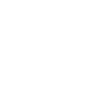
\includegraphics[draft,width=0.5\textwidth]{/sketch/placeholder}
%\caption{LeNet with various dropout values} 
%\label{fig:lenet_various_dropout}  
%\end{figure}



\begin{figure}[!htb]
\centering
\subfloat[Naive Dropout]{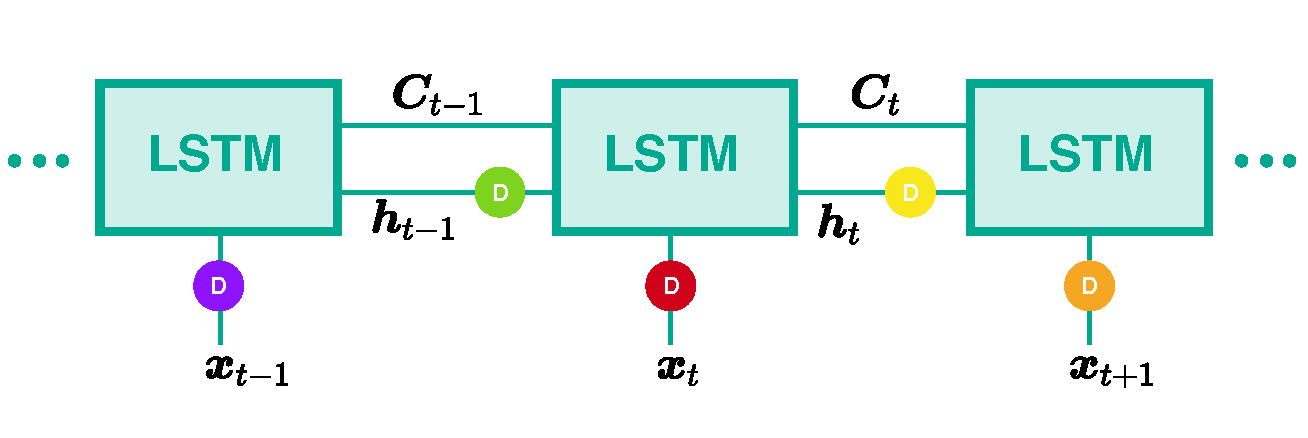
\includegraphics[width=0.8\textwidth]{sketch/lstm_naive_dropout} \label{fig:lstm_naive_dropout}} \\
\subfloat[Stationary Dropout]{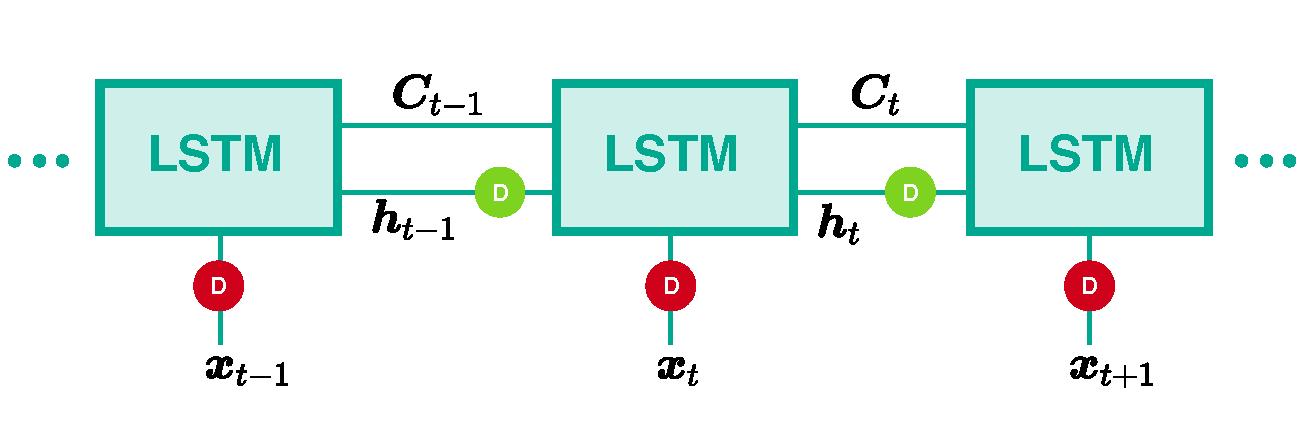
\includegraphics[width=0.8\textwidth]{sketch/lstm_variational_dropout} \label{fig:lstm_variational_dropout}}

\patcaption{LSTM with different dropout approaches.}{\textcircled{\tiny \textbf D} indicates a dropout mask and its color represents the suspension activity.}
\label{fig:dropout_lstm}
\end{figure}

However, unlike typical feedforward architectures, RNN layers are reused across time step, hence a question arises whether the same neurons in those layers should be suspended or they should be different neurons when applying the layers multiple times. \addfigure{\ref{fig:dropout_lstm}} illustrates these 2 different approaches where different colors represent different dropping activities. In particular, this stationary dropout was first proposed by \cite{GalTheoreticallyGroundedApplication2016} who applied  the technique to LSTM and GRU and found accuracy improvements on language modeling tasks.

\subsection{Proposal 2 : Gating units}
\begin{figure}[!htb]
\centering
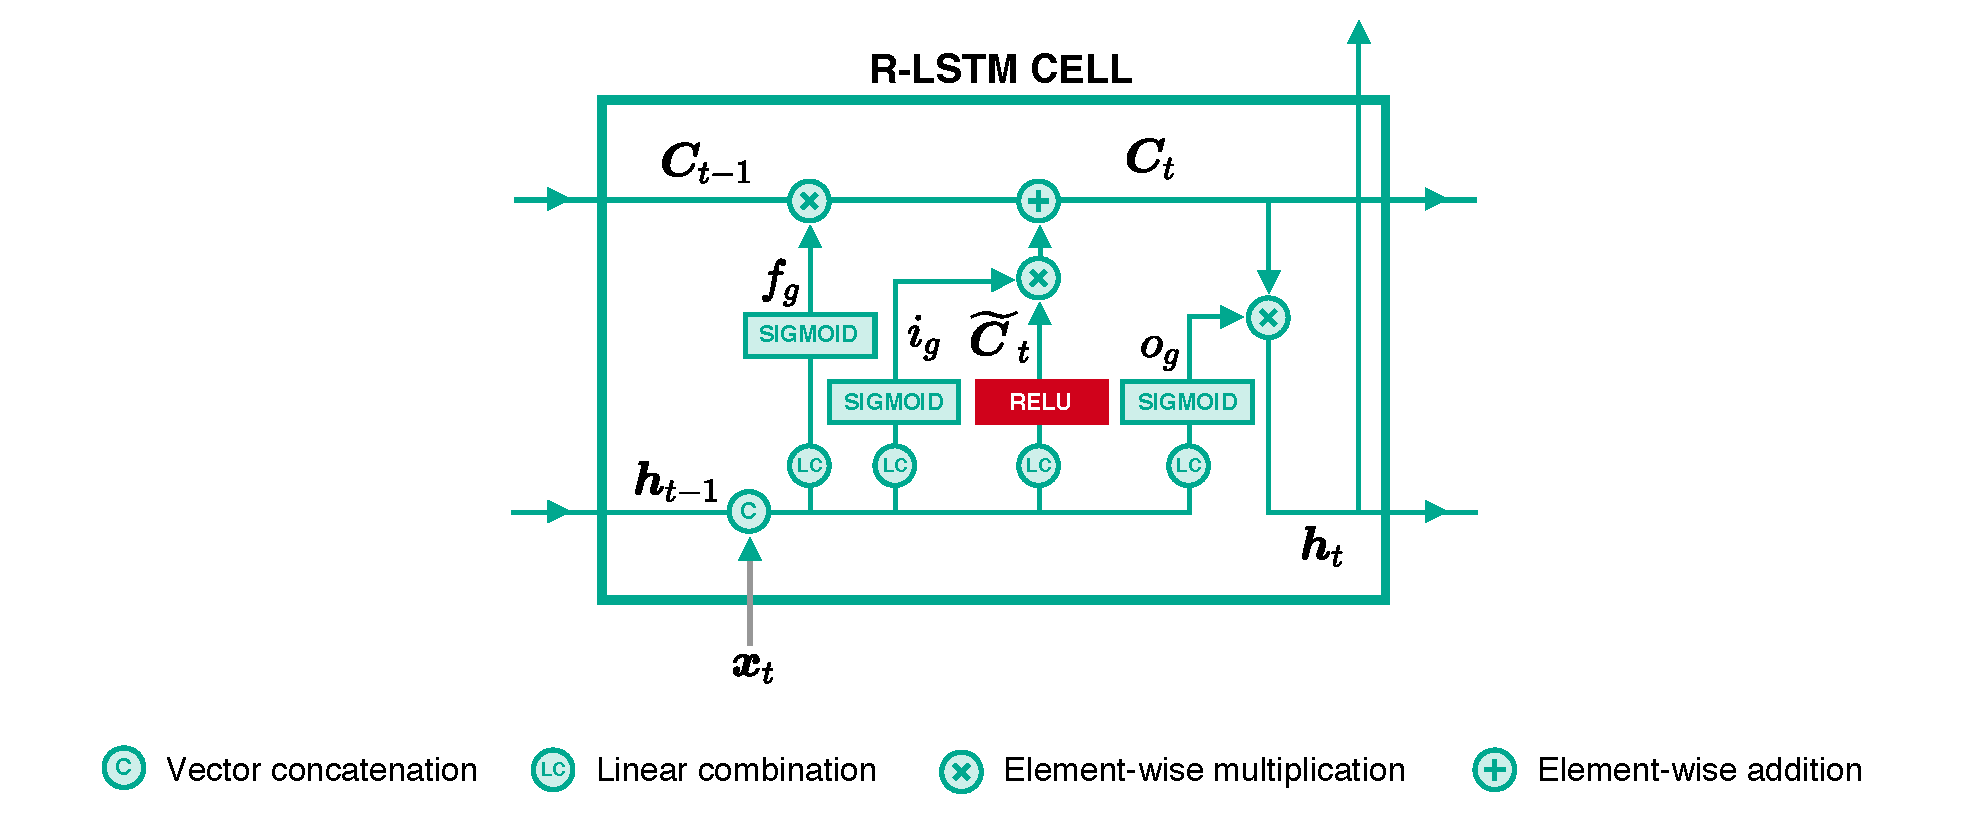
\includegraphics[width=1\textwidth]{sketch/relu_lstm}
\caption{R-LSTM Structure} 

\label{fig:relu_lstm} 
\end{figure}

It is already shown that gating units and addictive updates are critical mechanisms that enable LSTM to learn long term dependencies \cite{GreffLSTMsearchspace2017, Jozefowiczempiricalexplorationrecurrent2015a}. However, LSTM is not readily applicable for methods we are considering in this thesis. More precisely, the use of sigmoid and tanh activations violates the assumption of GB and DTD. Therefore, we propose a slight modified version of LSTM where ReLU activations are used to compute cell state candidates $\widetilde{C}_t$ instead of tanh functions. This results $C_t \in \mathbb{R}^+$, hence the tanh activation for $h_t$  is also removed.  Sigmoid activations are treated as constants when applying DTD and LRP, while its gradients are set to zero for GB. We refer this architecture as R-LSTM to differentiate from the original.  \addfigure{\ref{fig:relu_lstm}} presents an overview of R-LSTM architecture.


\subsection{Proposal 3 : Convolutional layer with literal connections}
As discussed in Section \ref{sec:conv}, convolution and pooling operator enable neural networks to learn hierarchical and invariant representations, which are directly beneficial to explanation quality. Because the \rnncell{ConvDeep} architecture we proposed in Section \ref{sec:exp2} does not seem to exploit this properly because it has recurrent connections only layers after the convolutional and pooling layers. This can be analogically viewed that the ConvDeep architecture only shares high-level features between step instead of low-level features. This might lead to obscure low-level features in the explanation. 

%In this proposal, we aims to share those low-level features to convolutional operators of the next step as well. We call this connections as \textit{literal connections} and   We are going to refer Conv$^+$ to the setting that employs convolutional layers with literal connections.


 \begin{figure}[!htb]
\centering
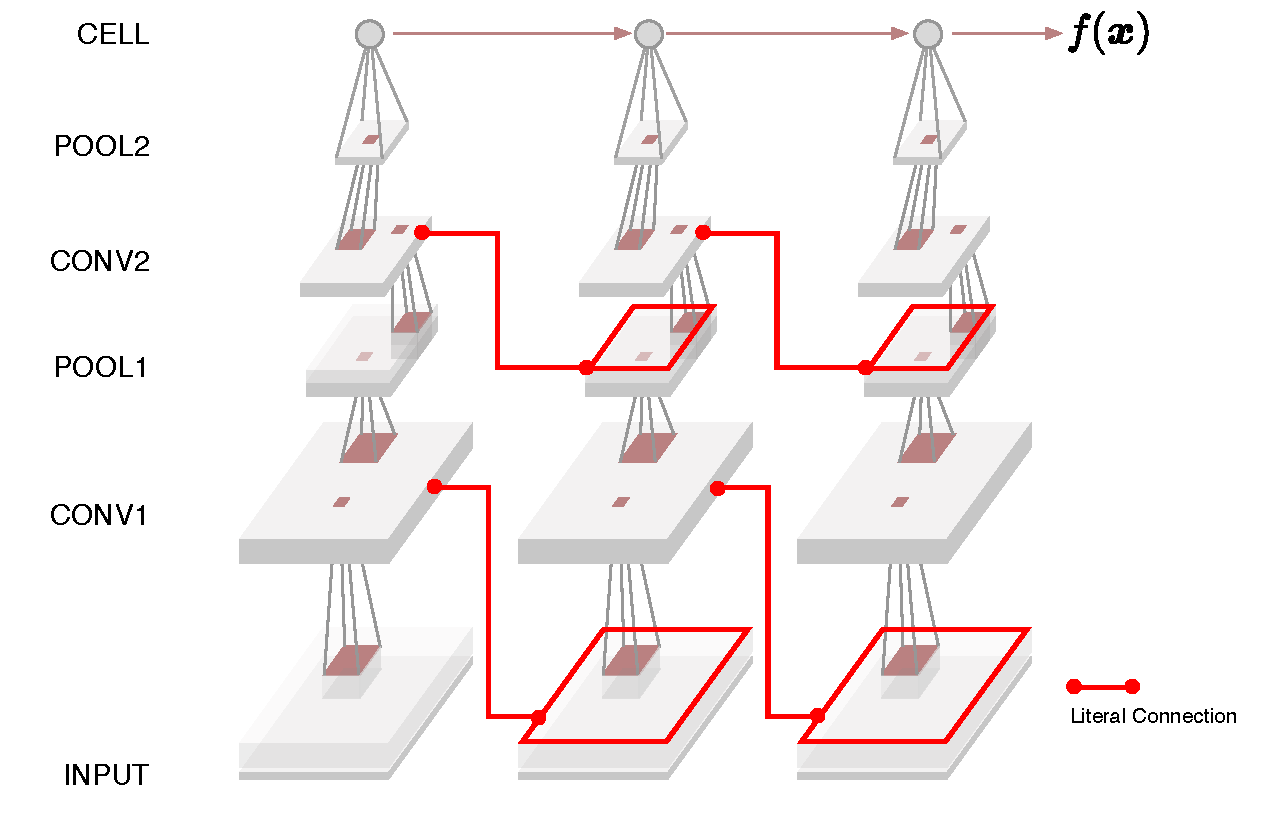
\includegraphics[width=\textwidth]{sketch/conv_literalconn}
\patcaption{ConvDeep with literal connections}{(\rnncell{Conv$^+$Deep}).} 
\label{fig:conv_literalconn}
\end{figure}

Therefore, we propose to also share results from convolution operators to the operators in the next step. We name this connections as \textit{literal connections} and \addfigure{\ref{fig:conv_literalconn}} illustrates such connections in red. From the following, we are going to refer Conv$^+$ to the setting where convolutional layers are connected through the literal connections. 

%\subsection{Setting}
In this experiment, we divided results into 2 parts. The first part focuses on stationary dropout and R-LSTM proposal and use the Deep architecture as a baseline. We refer models trained with stationary dropout with $-SD$ suffix. For R-LSTM's configuration, we also added one layer with 256 neurons between the input and 75 R-LSTM cells to make it comparable to the Deep architecture.  \todo{Figure X : show R-LSTM setting}

In the second part, we are going to discuss results from the literal connection proposal as well as results from ConvR-LSTM where the first fully-connected layer is replaced by convolutions and pooling layers with the same configuration as in ConvDeep. The number of R-LSTM cells is also the same to the first part. 

\todo{figure describe R-LSTM settings with cell?}


\subsection{Result}
Table \ref{tab:maj_exp3_model_acc} shows number of trainable parameters in the proposed architectures as well as accuracy.

\renewcommand{\arraystretch}{1.5}
\begin{table}[h]
\begin{center}
\begin{tabular}{lc|c|c|}
\cline{3-4}
& &
\multicolumn{2}{c|}{\parbox{3.5cm}{ \vskip 1mm \centering \textbf{Accuracy} \vskip 1mm}} \\ \hline
\multicolumn{1}{|l|}{\textbf{Cell architecture}} & \textbf{No. variables} & \textbf{MNIST-MAJ} & \textbf{FashionMNIST-MAJ} \\ \hline
\multicolumn{1}{|l|}{Deep-SD}                  & 153,578             & 98.10\% & 89.47\% \\ 
\multicolumn{1}{|l|}{R-LSTM}                    & 145,701   & 98.50\% & 91.35\% \\ 
\multicolumn{1}{|l|}{R-LSTM-SD}              &  145,701                & 98.57\% & 91.52\% \\ 
 \multicolumn{1}{|l|}{Conv$^+$Deep}       & 175,418                 & 97.92\% & 88.10\% \\
 \multicolumn{1}{|l|}{ConvR-LSTM-SD}      & 152,125                 & 99.35\% & 93.60\%  \\ 
\multicolumn{1}{|l|}{Conv$^+$R-LSTM-SD}   & 175,741                & 98.48\% & 88.19	\%  \\ \hline 
\end{tabular}

\end{center}
\caption{Number of trainable variables and model accuracy of the  proposed architectures for MNIST-MAJ and FashionMNIST-MAJ.}
\label{tab:maj_exp3_model_acc}
\end{table}
\renewcommand{\arraystretch}{1}


\subsubsection{Stationary Dropout and R-LSTM}
 \begin{figure}[!htb]
\centering
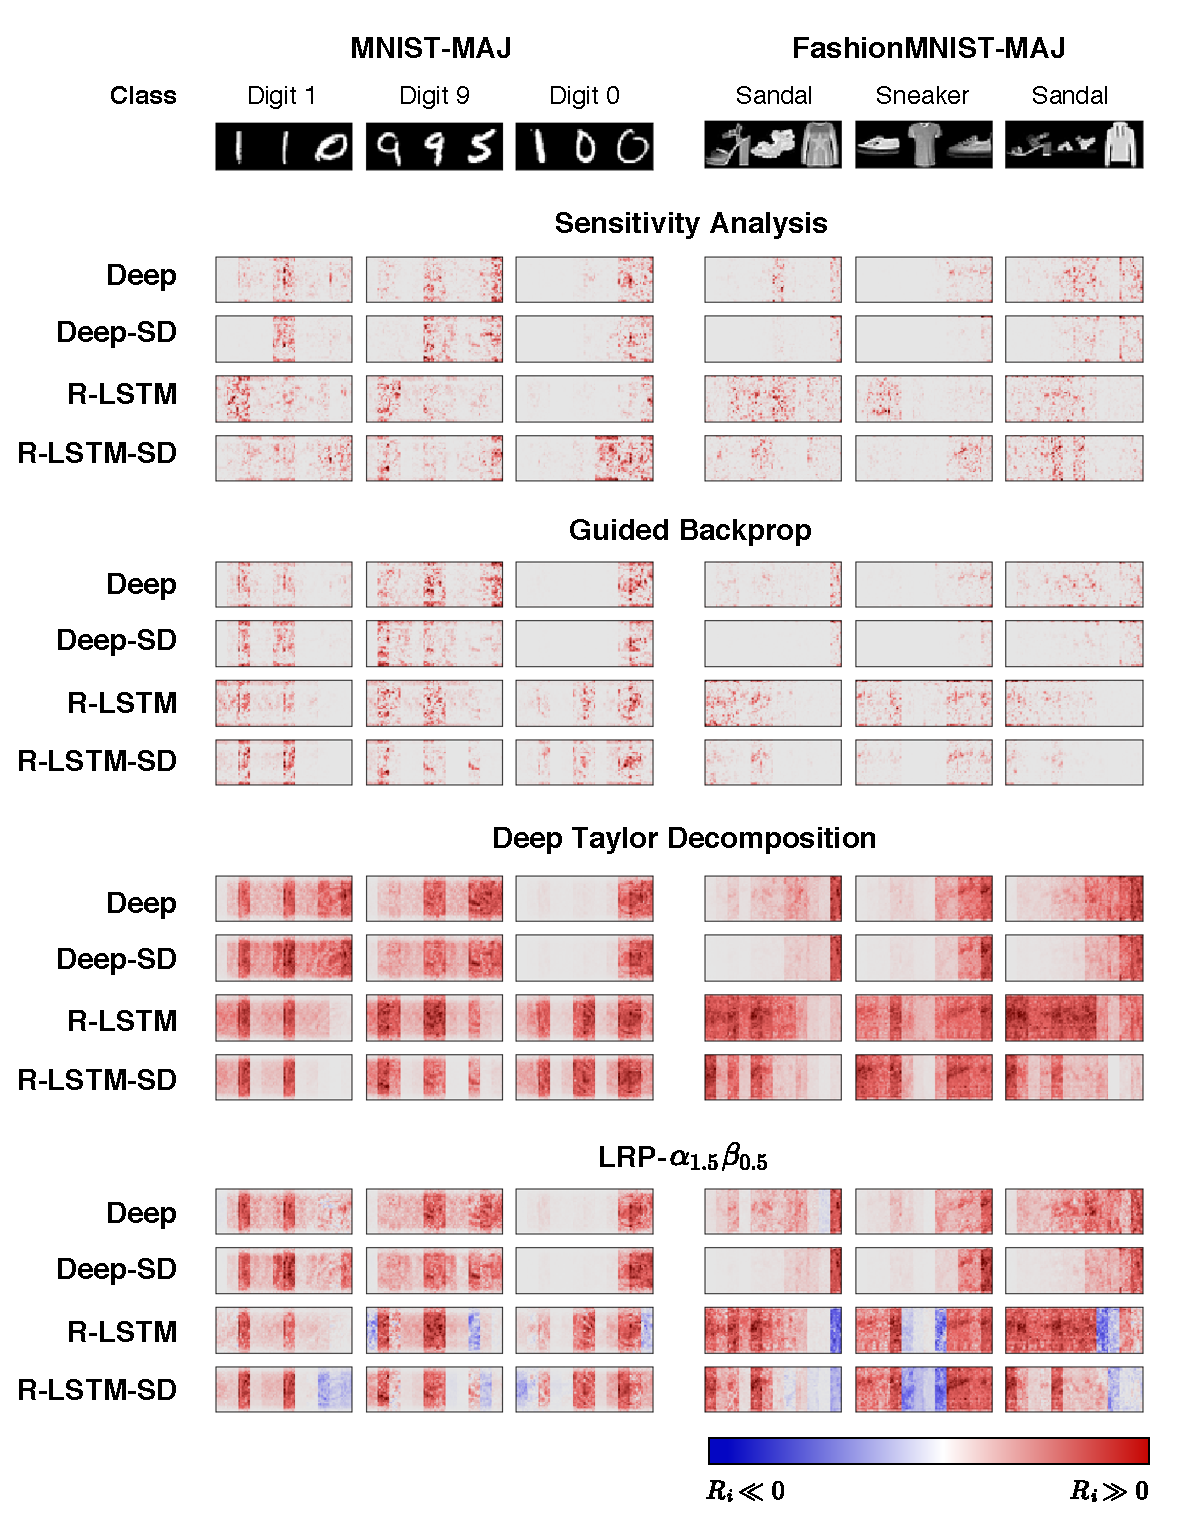
\includegraphics[width=\textwidth]{sketch/heatmap_msc_rlstm_exp}
\patcaption{Relevance heatmaps produced by different explanation techniques on Deep and R-LSTM architecture trained on MNIST-MAJ and FashionMNIST-MAJ with sequence length $T=12$ and different dropout configurations.}{\heatmapscaleexplain} 
\label{fig:heatmap_msc_rlstm_exp}
\end{figure}

\addfigure{\ref{fig:heatmap_msc_rlstm_exp}} shows results of the first part of this experiment. Here, variants of Deep and R-LSTM are compared. From the figure, it is obvious that R-LSTM provides better explanations than the Deep architecture. More precisely, we can directly observe the improvements from GB, DTD and $\lrpp$ heatmaps. Moreover, training with stationary dropout seems to produce R-LSTM with higher explanation capability. This is well notable on explanations from  DTD and $\lrpp$. In contrast, stationary dropout does not seem to have any prominent impact on the Deep architecture.


 \begin{figure}[!htb]
\centering
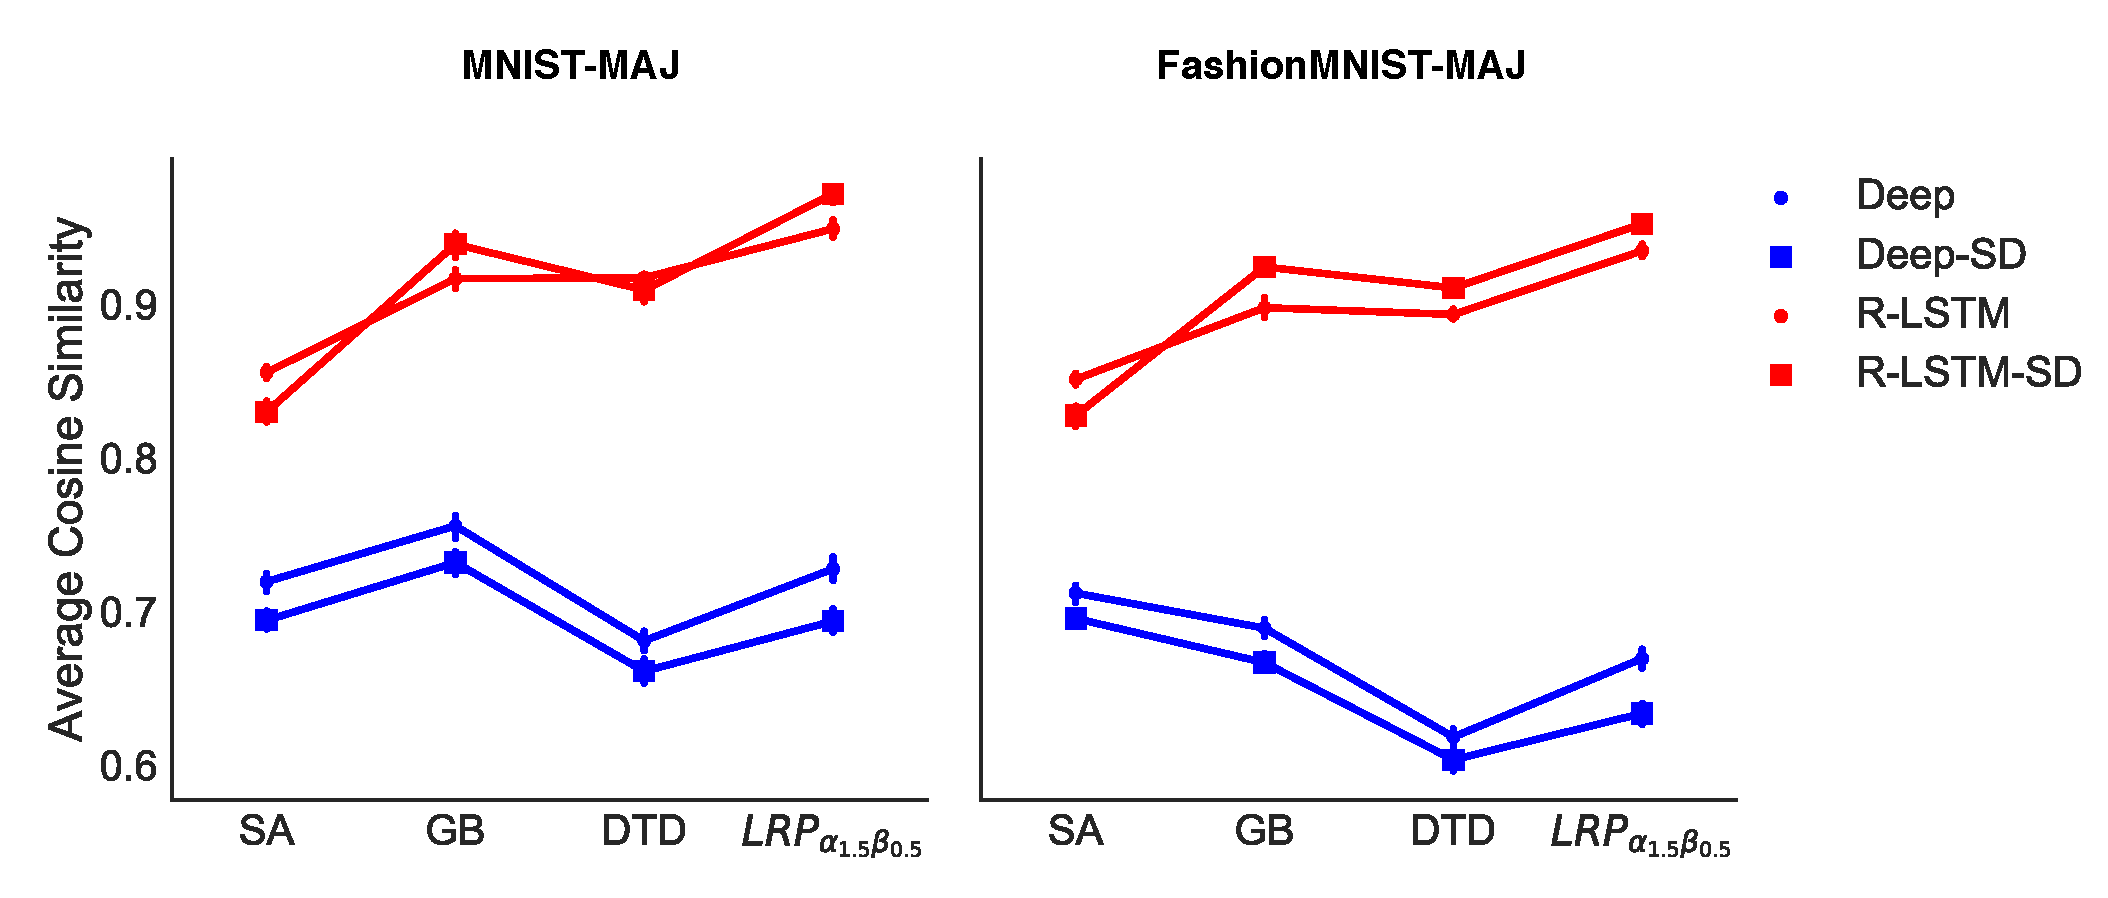
\includegraphics[width=\textwidth]{sketch/rel_dist_rlstm_exp}
%\caption{}  }. 
\patcaption{Average cosine similarity from different explanation techniques and Deep and R-LSTM architecture.}{The values are averaged from cross-validation results and the vertical lines depicted 95\% confidence interval. The baseline is the Deep architecture depicted by dotted blue line. Accuracy of the models can be found at Appendix  \ref{annex:model_acc}}

\label{fig:rel_dist_rlstm_exp}
\end{figure}

\addfigure{\ref{fig:rel_dist_rlstm_exp}} presents the quantitative evaluation. As a reminder, these plots are cosine similarity averaged over models trained with cross validation procedure described in  Section \ref{sec:evaluation_med}. The figure shows that R-LSTM significantly improves relevance distribution than the Deep architecture regardless of explanation techniques.  This means that R-LSTM is more explainable than the Deep architecture. Similar to one observation in Section \ref{sec:exp1_result}, we also see that the proportion of the improvement of DTD and LRP seem to have greater advantage from R-LSTM than the other methods.  

\addfigure{\ref{fig:rel_dist_rlstm_exp}}  also shows another interesting result. We can see that R-LSTM trained with stationary dropout, or R-LSTM-SD, produces better explanations than R-LSTM on FashionMNIST-MAJ, although the difference does not obvious on MNIST-MAJ. This might be due to complexity of FashionMNIST samples' structures, as a result keeping dropout mask the same for all step would enable the network to efficiently learn latent features from homogenous input. In contrast, this does not seem to be the case for the Deep architecture. Particularly, we find that the cosine similarity measurement of Deep-SD is lower than Deep in any case.

\todo{hypo thesis?}
\clearpage

\subsubsection{ConvDeep with literal connections and ConvR-LSTM}
 \begin{figure}[!htb]
\centering
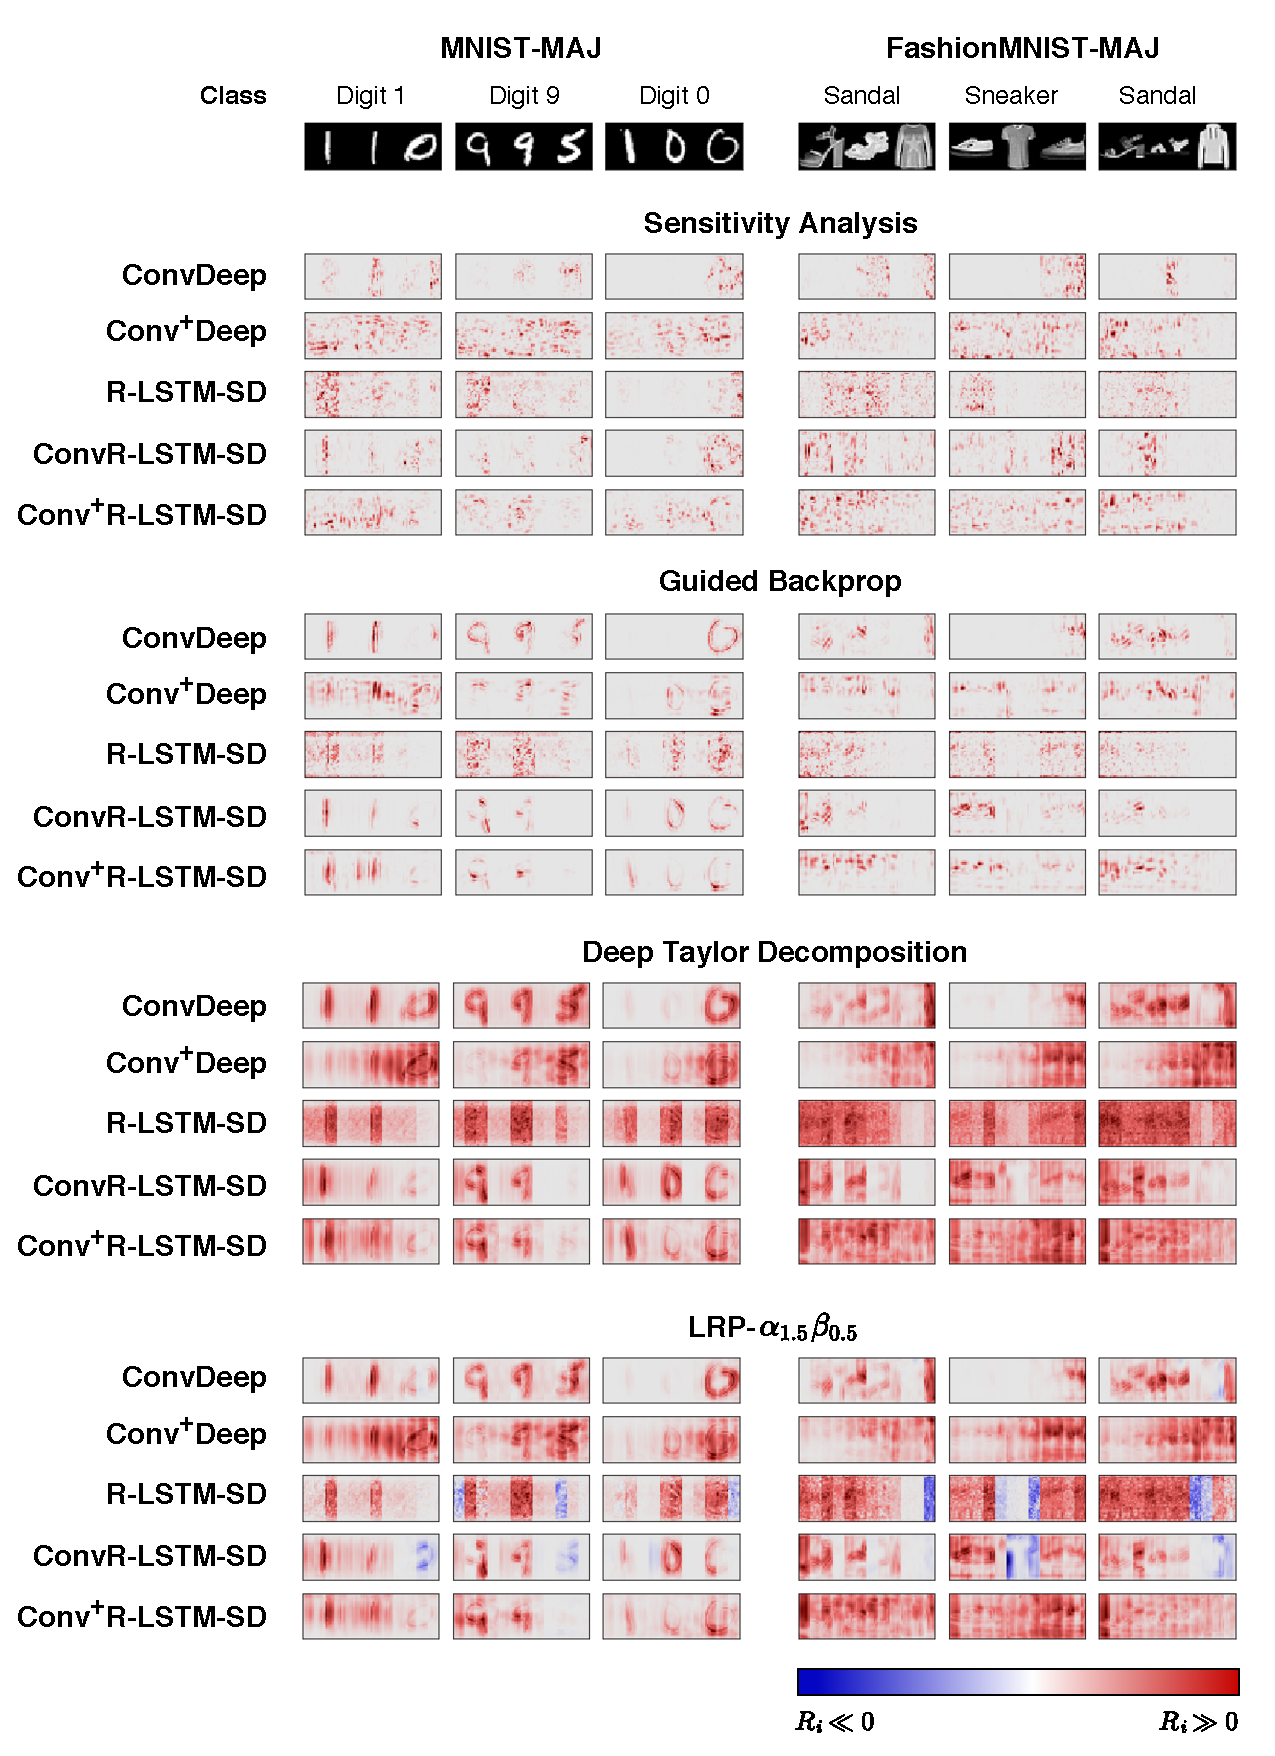
\includegraphics[width=\textwidth]{sketch/heatmap_msc_convtran_exp_v2}
\patcaption{Relevance heatmaps produced by different explanation techniques on variants of ConvDeep and R-LSTM architecture trained on MNIST-MAJ and FashionMNIST-MAJ with sequence length $T=12$.}{\heatmapscaleexplain} 
\label{fig:heatmap_msc_convtran_exp}
\end{figure}
For the second part, we compare the ConvDeep architecture and the effect of literal connections as well as R-LSTM-SD with convolutional layers, which is referred as ConvR-LSTM-SD. According to \addfigure{\ref{fig:heatmap_msc_convtran_exp}}, Conv$^+$Deep produces more diffuse relevance heatmaps than ConvDeep. This is specially notable on heatmaps from SA  and GB method. Similarly, Conv$^+$Deep also produces worse results for DTD and $\lrpp$, for example consider Digit 1 and Digit 9 sample, where the relevance scores are unnecessarily distributed to the last digit's block. 

\addfigure{\ref{fig:heatmap_msc_convtran_exp}} also shows relevance heatmaps from ConvR-LSTM-SD whose first fully-connected layer is replaced by 2 convolutional and pooling layers. Comparing to R-LSTM-SD, having convolutional and pooling layers does improve  the quality of the heatmaps further. In particular, we can clearly see samples' structures from the explanations. \addfigure{\ref{fig:heatmap_msc_convrlstm_pos_rel}} further emphasizes the improvement introduced by the convolutional and pooling layers. Here, we plots the relevance heatmaps by using only positive relevance. We can see that the heatmaps from ConvR-LSTM-SD are proper highlighted and provide substantial  features of the samples.

 \begin{figure}[!htb]
\centering
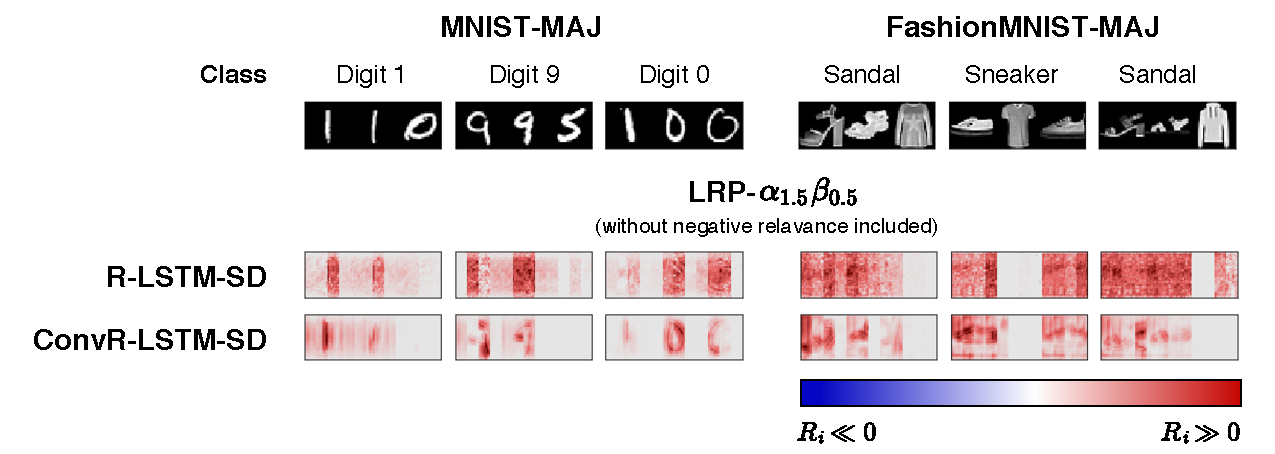
\includegraphics[width=\textwidth]{sketch/heatmap_msc_convrlstm_pos_rel}
\patcaption{Positive relevance heatmaps produced by $\lrpp$ technique on R-LSTM and ConvR-LSTM architecture trained on MNIST-MAJ and FashionMNIST-MAJ with sequence length $T=12$.}{\heatmapscaleexplain} 
\label{fig:heatmap_msc_convrlstm_pos_rel}
\end{figure}

 \begin{figure}[!htb]
\centering
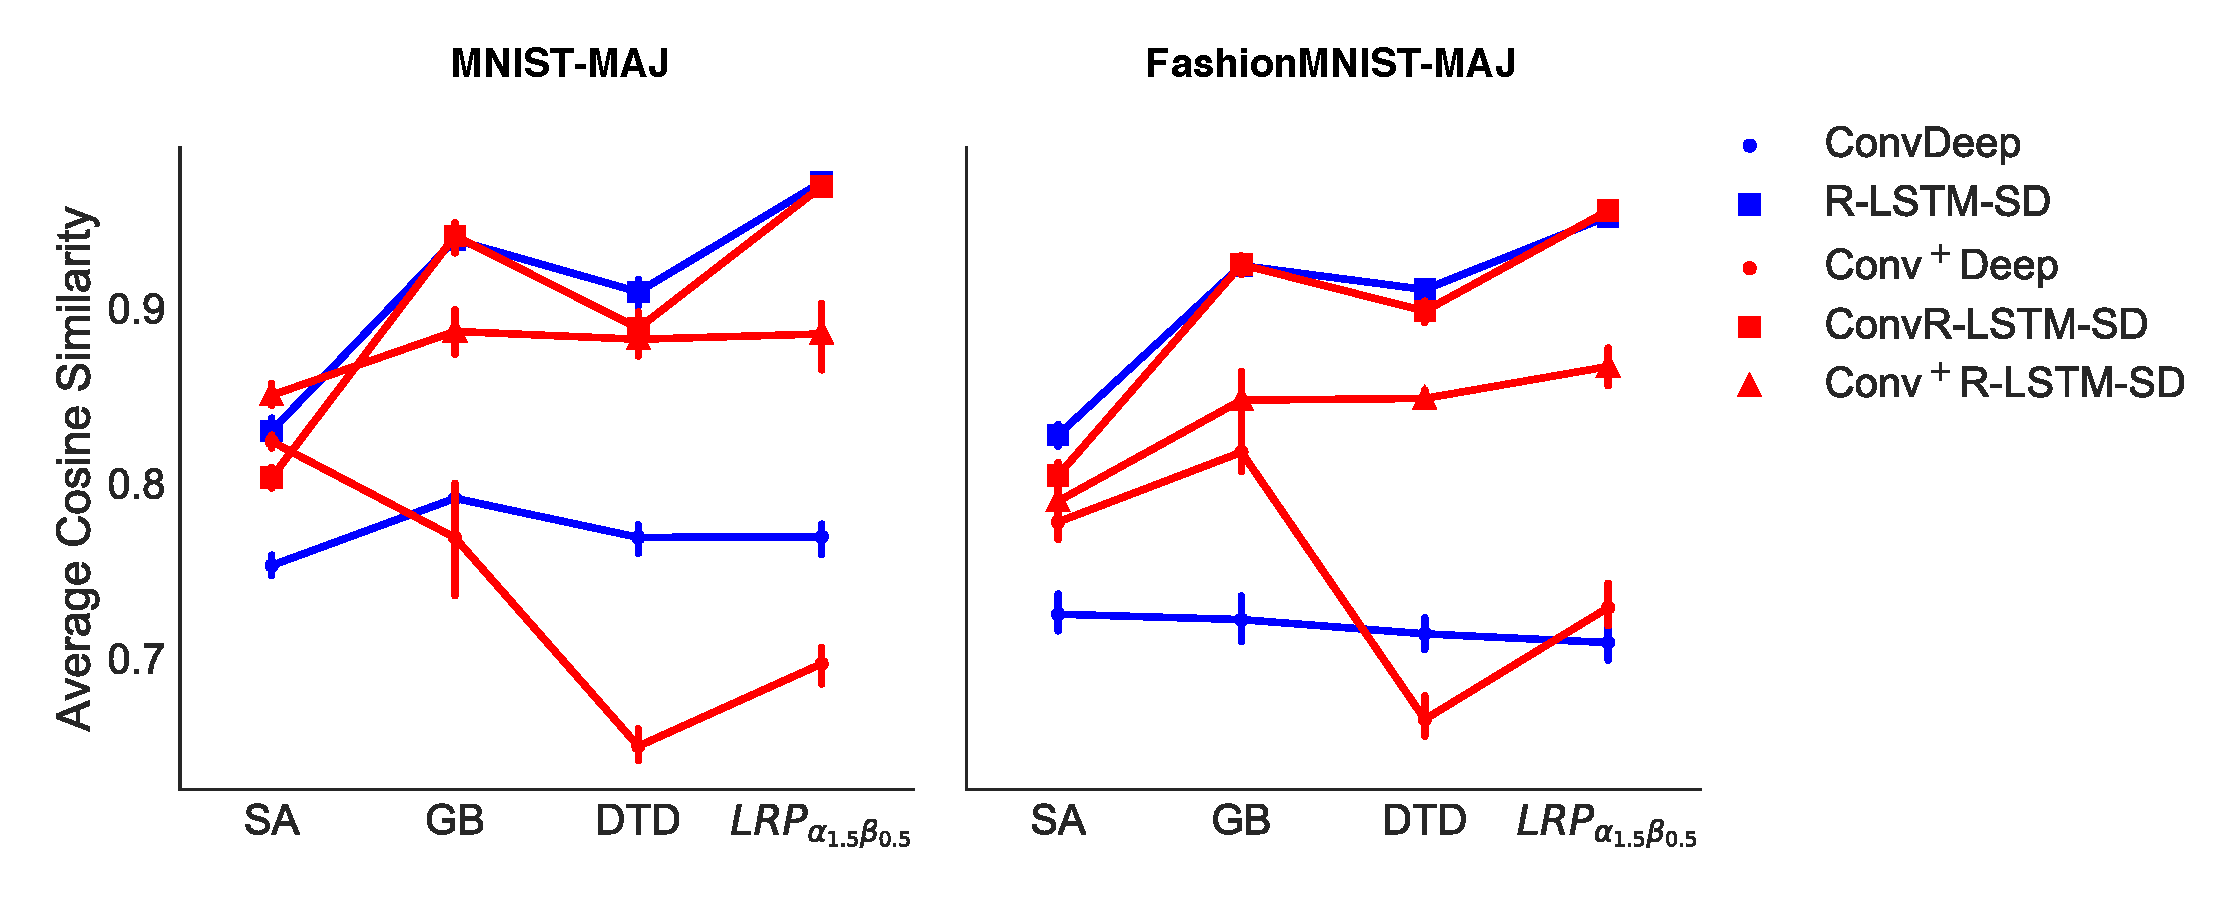
\includegraphics[width=\textwidth]{sketch/rel_dist_convdeep_trans_exp}
\patcaption{Average cosine similarity from different explanation techniques and variants of ConvDeep and R-LSTM architecture.}{The values are averaged from cross-validation results and the vertical lines depicted 95\% confidence interval. The baseline are the Deep and R-LSTM-SD architecture represented in blue. Accuracy of the models can be found at Appendix \ref{annex:model_acc}} 
\label{fig:rel_dist_convdeep_trans_exp}
\end{figure}

\addfigure{\ref{fig:rel_dist_convdeep_trans_exp}} presents the cosine similarity measurement this second part of the experiment. Here, ConvDeep and R-LSTM-SD are results from the previous experiments and used as baseline. Unexpectedly, having literal connections in ConvDeep does not seem to show consistent influence between MNIST-MAJ and FashionMNIST-MAJ. However, the connections considerably reduce the explanation capability of the ConvR-LSTM-SD architecture. 
 Although explanations from ConvR-LSTM-SD are less noisy and contain impressive structures from the input as shown in \addfigure{\ref{fig:heatmap_msc_convrlstm_pos_rel}}, the average cosine similarity of R-LSTM-SD and ConvR-LSTM-SD look almost identical. This is due to the fact our cosine similarity measurement operates on scalar values but not structures inside explanation heatmaps.
 
 \todo{hypo: In fact, using Tukey HSD test shows that the improvement is not statistically significant} 
\todo{hypothesis testing}

\clearpage

\subsection{Summary}
Results from this experiment shows some successful improvements from what we have seen on Sectoin \ref{sec:exp2}. In particular, employing gating unit and keeping dropout activities the same significantly improve explanation ability of RNN models on any explanation method.  

Moreover, convolutional and pooling layers enables the models to produce explanations with more perceivable input features than traditional fully-connected layers, although this improvement does not seem to be well captured by cosine similarity that we proposed to use. . This illustrates  a shortcoming of cosine similarity that we proposed to use for the quantitative evaluation.

On the other hand, literal connections do not show any consistent improvement for the settings we are considering. In fact, having wider confidence interval suggests that they seem to make explanations less stable.


%    \chapter{Implementation\label{cha:chapter5}}

This chapter describes the implementation of component X. Three systems were chosen as reference implementations: a desktop version for Windows and Linux PCs, a Windows Mobile version for Pocket PCs and a mobile version based on Android. 

\section{Environment\label{sec:env}}
The following software, respectively operating systems, were used for the implementation:

\begin{itemize}
		\item Windows XP and Ubuntu 6
		\vspace{-0.1in} 
		\item Java Development Kit (JDK) 6 Update 10 
		\vspace{-0.1in} 
		\item Eclipse Ganymede 3.4
		\vspace{-0.1in} 
		\item Standard Widget Toolkit 3.4
\end{itemize}

\section{Project Structure\label{sec:projectstructure}}

The implementation is seperated into 2 distinguished eclipse projects as depicted in figure \ref{fig:projects}.

\begin{figure}[htb]
  \centering
  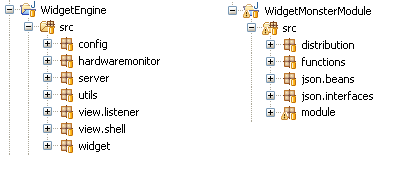
\includegraphics[width=10cm]{screenshot_2_projects}
  \caption{Project Structure}
  \label{fig:projects}
\end{figure}

\noindent
The following listing briefly describes the single packages of both projects in alphabetical order to give an overview of the implementation:
\\
\\
\textbf{config} 
\\
Lorem Ipsum...
\\
\\
\textbf{server} 
\\
Lorem Ipsum...
\\
\\
\textbf{utils} 
\\
Lorem Ipsum...

\section{Important Implementation Aspects\label{sec:gui}}

Do not explain every class in detail. Give a short introduction about the modules or the eclipse projects. If you want to explain relevant code snippets use the 'lstlisting' tag of LaTeX. Put only short snippets into your thesis. Long listing should be part of the annex.

\lstset{caption=JSON String Code Snippet,label=jsonstring,showstringspaces=false}
\begin{lstlisting}
{
	id: 1,
	method: "myInstance.getGroup",
	params: ["Teammates", 2, true]
}

{
	id: 2,
	result: [
		  "groupDesc":"These are my teammates",
		  {
			"javaClass":"src.package.MemberClass",
			"memberName": "Bob",      
		  }
		]
}\end{lstlisting}

You can also compare different approaches. Example: Since the implementation based on X failed I choosed to implement the same aspect based on Y. The new approach resulted in a much faster ...

\section{Graphical User Interface\label{sec:gui}}

Lorem Ipsum...

\section{Documentation\label{sec:docu}}

Lorem Ipsum...



%    \chapter{Evaluation\label{cha:chapter6}}

In this chapter the implementation of Component X is evaluated. An example instance was created for every service. The following chapter validates the component implemented in the previous chapter against the requirements.
\\
\\
Put some screenshots in this section! Map the requirements with your proposed solution. Compare it with related work. Why is your solution better than a concurrent approach from another organization?

\section{Test Environment\label{sec:testenvir}}

Fraunhofer Institute FOKUS' Open IMS Playground was used as a test environment for the telecommunication services. The IMS Playground ...

\section{Scalability\label{sec:scal}}

Lorem Ipsum

\section{Usability\label{sec:usab}}

Lorem Ipsum

\section{Performance Measurements\label{sec:performance}}

Lorem Ipsum
%    \chapter{Conclusion\label{cha:chapter7}}
The final chapter summarizes the thesis. The first subsection outlines the main ideas behind Component X and recapitulates the work steps. Issues that remained unsolved are then described. Finally the potential of the proposed solution and future work is surveyed in an outlook.

\section{Summary\label{sec:summary}}

Explain what you did during the last 6 month on 1 or 2 pages!
\\
\\
\noindent The work done can be summarized into the following work steps

\begin{itemize}
		\item Analysis of available technologies
		\vspace{-0.11in} 
		\item Selection of 3 relevant services for implementation
		\vspace{-0.11in} 
		\item Design and implementation of X on Windows
		\vspace{-0.11in} 
		\item Design and implementation of X on mobile devices
		\vspace{-0.11in} 
		\item Documentation based on X
		\vspace{-0.11in} 
		\item Evaluation of the proposed solution
\end{itemize}

\section{Dissemination\label{sec:dissemination}}

Who uses your component or who will use it? Industry projects, EU projects, open source...? Is it integrated into a larger environment? Did you publish any papers?

\section{Problems Encountered\label{sec:problems}}

Summarize the main problems. How did you solve them? Why didn't you solve them?

\section{Outlook\label{sec:outlook}}

Future work will enhance Component X with new services and features that can be used ...

% ---------------------------------------------------------------
\backmatter % no page numbering from here
%    \addchap{List of Acronyms}

\begin{tabbing}
spacespacespace \= space \kill

Adam \> Adaptive Moment Estimation \\
CNN \> Convolutional Neural Networks \\
DTD \> deep Taylor decomposition \\
GB  \> guided backprop \\
LRP \> Layer-Wise Relevance Propagation \\
MT \> Machine Translation \\
NLP \> Natural Language Processing \\
NN \> Neural Networks \\
RNN \> Recurrent Neural Networks \\
SA  \> sensitivity analysis \\

%3GPP	 \> 	3rd Generation Partnership Project	 \\
%AJAX	\>	Asynchronous JavaScript and XML \\
%API	 \> 	Application Programming Interface	 \\
%AS	\>	Application Server \\
%CSCF	 \> 	Call Session Control Function	 \\
%CSS	\>	Cascading Stylesheets \\
%DHTML	\>	Dynamic HTML \\
%DOM	\>	Document Object Model \\
%FOKUS	\>	Fraunhofer Institut fuer offene Kommunikationssysteme \\
%GUI	\>	Graphical User Interface \\
%GPS	\>	Global Positioning System \\
%GSM	\>	Global System for Mobile Communication\\
%HTML	\>	Hypertext Markup Language \\
%HSS	 \> 	Home Subscriber Server	 \\
%HTTP	 \> 	Hypertext Transfer Protocol	 \\
%I-CSCF	 \> 	Interrogating-Call Session Control Function	 \\
%IETF	\>	Internet Engineering Task Force \\
%IM	\>	Instant Messaging \\
%IMS	 \> 	IP Multimedia Subsystem	 \\
%IP	 \> 	Internet Protocol	 \\
%J2ME	\>	Java Micro Edition \\
%JDK	\>	Java Developer Kit \\
%JRE	\>	Java Runtime Environment \\
%JSON	\>	JavaScript Object Notation \\
%JSR	\>	Java Specification Request \\
%JVM	 \> 	Java Virtual Machine	 \\
%NGN	 \> 	Next Generation Network	 \\
%OMA	 \> 	Open Mobile Alliance	 \\
%P-CSCF	 \> 	Proxy-Call Session Control Function	 \\
%PDA	\>	Personal Digital Assistant \\
%PEEM	 \> 	Policy Evaluation, Enforcement and Management	 \\
%QoS	 \> 	Quality of Service	 \\
%S-CSCF	 \> 	Serving-Call Session Control Function	 \\
%SDK	\>	Software Developer Kit \\
%SDP	\>	Session Description Protocol \\
%SIP	 \> 	Session Initiation Protocol	 \\
%SMS	\>	Short Message Service \\
%SMSC	\> Short Message Service Center \\
%SOAP	 \> 	Simple Object Access Protocol	 \\
%SWF	\>	Shockwave Flash \\
%SWT	\>	Standard Widget Toolkit \\
%TCP	 \> 	Transmission Control Protocol	 \\
%Telco API	\>	Telecommunication API \\
%TLS	\>	Transport Layer Security \\
%UMTS	 \> 	Universal Mobile Telecommunication System	 \\
%URI	 \> 	Uniform Resource Identifier	 \\
%VoIP	 \> 	Voice over Internet Protocol	 \\
%W3C	 \> 	World Wide Web Consortium	 \\
%WSDL	\>	Web Service Description Language \\
%XCAP	 \> 	XML Configuration Access Protocol	 \\
%XDMS	 \> 	XML Document Management Server	 \\
%XML	 \> 	Extensible Markup Language	 \\
\end{tabbing}
\endinput

		
		% if you want to provide a glossary with explanations of important terms put it in here

%    \bibliographystyle{geralpha}
    \bibliographystyle{apalike}
    \bibliography{./bib/references}
    
%    \addchap{Appendix}

\begin{appendix}

\todo{appendix : all architectures that aren't desribed with no. neurons}

\todo{appendix : list of model accuracy and variance for hypothesis testing}

%\begin{figure}
%
%\caption{Hypothesis testing result for Experiment 1}
%\label{annex:hypo_exp1}
%\end{figure}

\lstset{captionpos=t,showstringspaces=false, basicstyle={\fontfamily{pcr}\selectfont\footnotesize}}

\lstinputlisting[label={annex:hypo_exp1}, caption={Hypothesis testing results of Section \ref{sec:exp2}}]{hypothesis-testing-results/exp1.txt}

\end{appendix}

\endinput


\end{document}
x